\chapter{Linear regression models}
\label{c_regression}

\section{Introduction}
\label{s_regression_intro}

This chapter continues the theme of analysing statistical associations
between variables. The methods described here are appropriate when the
response variable $Y$ is a continuous, interval level variable. We
will begin by considering bivariate situations where the only explanatory variable
$X$ is also a continuous variable. Section \ref{s_regression_descr}
first discusses graphical and numerical descriptive techniques for this
case, focusing on two very commonly used tools: a \emph{scatterplot} of
two variables, and a measure of association known as the
\emph{correlation} coefficient. Section \ref{s_regression_simple} then
describes methods of statistical inference for associations between two
continuous variables. This is done in the context of a statistical model
known as the \emph{simple linear regression model}.

The ideas of simple linear regression modelling can be extended to a
much more general and powerful set methods known as \emph{multiple
linear regression models}.
These can have several explanatory
variables, which makes it possible to examine associations between any
explanatory variable and the response variable, while controlling for
other explanatory variables.
An important reason for the usefulness of
these models is that they play a key role in statistical analyses
which correspond to research questions that are causal in nature.
As an interlude, we discuss issues of causality in research design and
analysis briefly in Section \ref{s_regression_causality}.
Multiple linear models are then
introduced in Section
\ref{s_regression_multiple}.
The models can also include categorical
explanatory variables with any number of categories, as explained in
Section \ref{s_regression_dummies}.

The following example will be used for illustration throughout this
chapter:

\textbf{Example 8.1: Indicators of Global Civil Society}
\label{p_civilsoc}

The \emph{Global Civil Society 2004/5} yearbook gives tables of a range
of characteristics of the countries of the world\footnote { Anheier, H.,
Glasius, M.\ and Kaldor, M.\ (eds.) (2005). \emph{Global Civil Society
2004/5}. London: Sage. The book gives detailed references to the
indices considered here. Many thanks to Sally Stares for providing the
data in an electronic form.}. The following measures will be considered
in this chapter:
\begin{itemize}
\item
Gross Domestic Product (\textbf{GDP}) per capita in 2001
(in current international dollars,
adjusted for purchasing power parity)
\item
\textbf{Income level} of the country
in three groups used by the Yearbook, as
Low income, Middle income or High income
\item
\textbf{Income inequality} measured by the Gini index (with 0
representing perfect equality and 100 perfect inequality)
\item
A measure of \textbf{political rights and civil liberties} in 2004, obtained as
the average of two indices for these characteristics produced by the
Freedom House organisation (1 to 7, with higher values indicating more
rights and liberties)
\item
World Bank Institute's measure of control of \textbf{corruption} for 2002
(with high values indicating low levels of corruption)
\item
Net \textbf{primary school enrolment} ratio 2000-01 (\%)
\item
\textbf{Infant mortality rate} 2001 (\% of live births)
\end{itemize}
We will discuss various associations between these variables. It should
be noted that the analyses are mainly illustrative examples, and the
choices of explanatory and response variables do not imply any strong
claims about causal connections between them. Also, the fact that
different measures refer to slightly different years is ignored; in
effect, we treat each variable as a measure of ``recent'' situation in
the countries. The full data set used here includes  165 countries. Many
of the variables are not available for all of them, so most of the
analyses below use a smaller number of countries.

\section[Associations between continuous variables]
{Describing association between two continuous variables}
\label{s_regression_descr}

\subsection{Introduction}
\label{ss_regression_descr_intro}

Suppose for now that we are considering data on two continuous
variables. The descriptive techniques discussed in this section do not strictly
speaking require a distinction between an explanatory variable and a
response variable, but it is nevertheless useful in many if not most
applications. We will reflect this in the notation by denoting the
variables $X$ (for the explanatory variable) and $Y$ (for the
response variable). The observed data consist of the pairs of
observations $(X_{1}, Y_{1}), (X_{2}, Y_{2}), \dots, (X_{n}, Y_{n})$ of
$X$ and $Y$ for each of the $n$ subjects in a sample, or, with more
concise notation, $(X_{i}, Y_{i})$ for $i=1,2,\dots,n$.

We are interested in analysing the association between $X$ and $Y$.
Methods for \emph{describing} this association in the
sample are first described in this section, initially with some standard graphical
methods in Section \ref{ss_regression_descr_plots}. This leads to a
discussion in Section \ref{ss_regression_descr_assoc} of what we
actually mean by associations in this context, and then to a definion of
numerical summary measures for such associations in Section
\ref{ss_regression_descr_corr}. Statistical \emph{inference} for the
associations will be considered in Section \ref{s_regression_simple}.

\subsection{Graphical methods}
\label{ss_regression_descr_plots}

\subsubsection{Scatterplots}

The standard statistical graphic for summarising the association between
two continuous variables is a \textbf{scatterplot}. An example of it is
given in Figure \ref{f_corruption1}, which shows a scatterplot of
Control of corruption against GDP per capita for 61 countries for which
the corruption variable is at least 60 (the motivation of this
restriction will be discussed later). The two axes of the plot show
possible values of the two variables. The horizontal axis, here
corresponding to Control of corruption, is conventionally used for the
explanatory variable $X$, and is often referred to as the
\textbf{X-axis}. The vertical axis, here used for GDP per capita, then
corresponds to the response variable $Y$, and is known as the
\textbf{Y-axis}.

\begin{figure}
\caption{A scatterplot of Control of corruption vs.\ GDP per capita in
the Global Civil Society data set, for 61 countries with Control of
corruption at least 60. The dotted lines are drawn to the point
corresponding to the
United Kingdom.}
\label{f_corruption1}

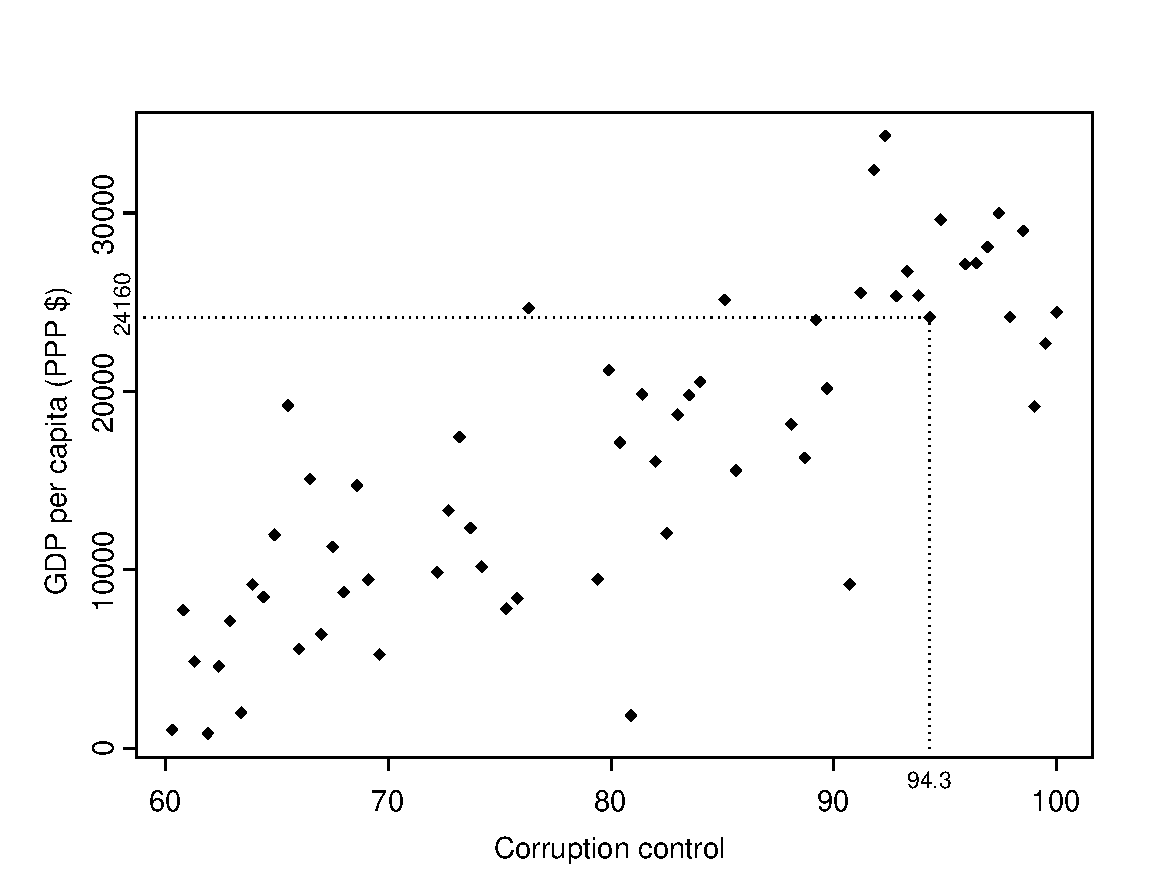
\includegraphics[width=14cm]{corruption1}

\end{figure}

The observed data are shown as points in the scatterplot, one for each
of the $n$ units. The location of each point is determined by its values
of $X$ and $Y$. For example, Figure \ref{f_corruption1} highlights the
observation for the United Kingdom, for which the corruption measure
($X$) is 94.3 and GDP per capita ($Y$) is \$24160. The point for UK is
thus placed at the intersection of a vertical line drawn from 94.3 on
the $X$-axis and a horizontal line from 24160 on the $Y$-axis, as shown
in the plot.

The principles of good graphical presentation on clear labelling,
avoidance of spurious decoration and so on (c.f.\ Section
\ref{s_descr1_presentation}) are the same for scatterplots as for any
statistical graphics. Because the crucial visual information in a
scatterplot is the shape of the cloud of the points, it is now often not
necessary for the scales of the axes to begin at zero, especially if
this is well outside the ranges of the observed values of the variables
(as it is for the $X$-axis of Figure \ref{f_corruption1}). Instead, the
scales are typically selected so that the points cover most of the
plotting surface. This is done by statistical software,
but there are many situations were it is advisable to overrule the
automatic selection (e.g.\ for making scatterplots of the same variables
in two different samples directly comparable).

The main purpose of a scatterplot is to examine possible associations
between $X$ and $Y$. Loosely speaking, this means considering the shape
and orientation of the cloud of points in the graph. In Figure
\ref{f_corruption1}, for example, it seems that most of the points are
in a cluster sloping from lower left to upper right. This indicates that
countries with low levels of Control of corruption (i.e.\ high levels of
corruption itself) tend to have low GDP per capita, and those with
little corruption tend to have high levels of GDP. A more careful
discussion of such associations again relates them to the formal definition
in terms of conditional distributions, and also provides a basis for the
methods of inference introduced later in this chapter. We will resume
the discussion of these issues in Section
\ref{ss_regression_descr_assoc} below. Before that, however, we will
digress briefly from the main thrust of this chapter in order to
describe a slightly different kind of scatterplot.

\subsubsection{Line plots for time series}

A very common special case of a scatterplot is
one where the observations correspond to measurements of a variable for
the same unit at several occasions over time. This is illustrated by the
following example (another one is Figure \ref{f_houseprices} on page
\pageref{f_houseprices}):

\emph{Example: Changes in temperature, 1903--2004}

Figure \ref{f_temperatures} summarises data on average annual
temperatures over the past century in five locations. The data were
obtained from the GISS Surface Temperature (GISTEMP) database maintained
by the NASA Goddard Institute for Space Studies\footnote{Accessible at
\texttt{data.giss.nasa.gov/gistemp/}. The temperatures used
here are those listed in the data base under ``after combining sources
at same location''.}. The database contains time series of average
monthly surface temperatures from several hundred meterological stations
across the world. The five sites considered here are Haparanda in
Northern Sweden, Independence, Kansas in the USA, Choshi on the east
coast of Japan, Kimberley in South Africa, and the Base Orcadas Station
on Laurie Island, off the coast of Antarctica. These were chosen rather
haphazardly for this illustration, with the aim of obtaining a
geographically scattered set of rural or small urban locations (to avoid
issues with the heating effects of large urban areas). The temperature
for each year at each location is here recorded as the difference from the
temperature at that location in 1903\footnote{More specifically, the differences
are between 11-year \emph{moving averages}, where each year is
represented by the average of the temperature for that year and the five
years before and five after it (except at the ends of the series, where
fewer observations are used). This is done to smooth out short-term
fluctuations from the data, so that longer-term trends become more
clearly visible.}.

\begin{figure}[t]
\caption{Changes of average annual temperature (11-year moving averages)
from 1903 in five locations. See the text for further details.}
\label{f_temperatures}
\begin{center}
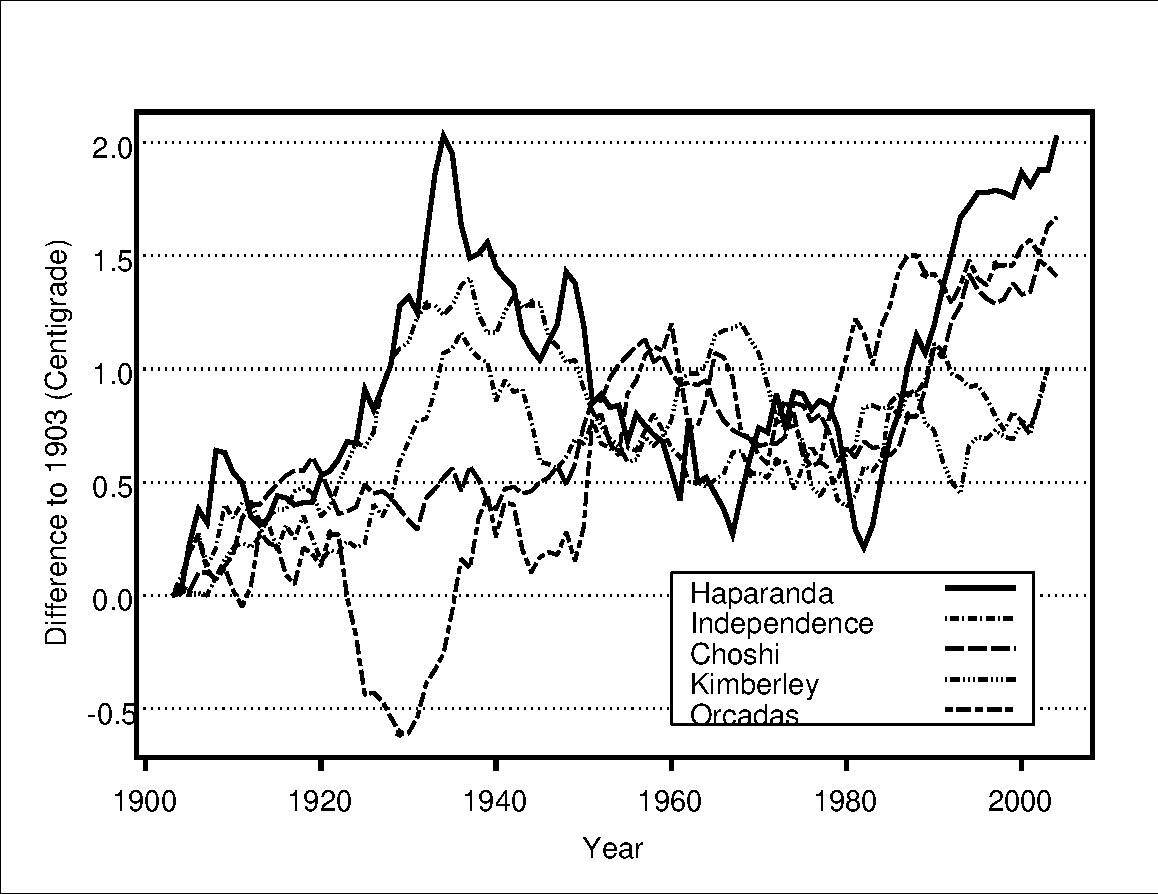
\includegraphics[width=13cm]{temperplot}\\
\footnotesize{Source: The GISTEMP database
(\texttt{data.giss.nasa.gov/gistemp/})}
\end{center}

\end{figure}

Consider first the data for Haparanda only. Here we have two variables,
year and temperature, and 102 pairs of observations of them, one for
each year between 1903 and 2004. These pairs could now be plotted in a
scatterplot as described above. Here, however, we can go further to
enhance the visual effect of the plot. This is because the observations
represent measurements of a variable (temperature difference) for
the same unit (the town of Haparanda) at several successive times
(years). These 102 measurements form a \emph{time series} of temperature
differences for Haparanda over 1903--2004. A standard graphical trick
for such series is to connect the points for successive times by
lines, making it easy for the eye to follow the changes over time in the
variable on the $Y$-axis. In Figure \ref{f_temperatures} this is done
for Haparanda using a solid line. Note that doing this would make no
sense for scatter plots like the one in Figure \ref{f_corruption1}, because
all the points there represent different subjects, in that case countries.

We can easily include several such series in the
same graph. In Figure \ref{f_temperatures} this is done by plotting the
temperature differences for each of the five locations using different
line styles. The graph now summarises data on three variables, year,
temperature and location. We can then examine changes over time for any
one location, but also compare patterns of changes between them. Here
there is clearly much variation within and between locations, but also
some common features. Most importantly, the
temperatures have all increased over the past century. In all five
locations the average annual temperatures at the end of the period were
around 1--2$^{\circ}$C higher than in 1903.

A set of time series like this is an example of dependent data in the
sense discussed in Section \ref{s_means_dependent}. There we considered
cases with pairs of observations, where the two observations in each
pair had to be treated as statistically dependent. Here all of the
temperature measurements for one location are dependent, probably
with strongest dependence between adjacent years and less dependence
between ones further apart. This means that we will not be able to
analyse these data with the methods described later in this chapter,
because these assume statistically independent observations. Methods of
statistical modelling and inference for dependent data of the kind
illustrated by the temperature example are beyond the scope of this
course. This, however, does not prevent us from using a plot like Figure
\ref{f_temperatures} to \emph{describe} such data.

\subsection{Linear associations}
\label{ss_regression_descr_assoc}

Consider again statistically independent observations of $(X_{i},
Y_{i})$, such as those displayed in Figure \ref{f_corruption1}. Recall
the definition that two variables are
associated if the conditional distribution of $Y$ given $X$ is different
for different values of $X$. In the two-sample
examples of Chapter \ref{c_means}
this could be examined by comparing two conditional distributions, since
$X$ had only two possible values. Now, however, $X$ has many (in
principle, infinitely many) possible values, so we will need to somehow
define and compare conditional distributions given each of them. We
will begin with a rather informal discussion of how this might be done.
This will lead directly to a more precise and formal definition
introduced in Section \ref{s_regression_simple}.


\begin{figure}[t]
\caption{
The same scatterplot of Control of corruption vs.\ GDP per capita as in
Figure \ref{f_corruption1}, augmented by the best-fitting (least
squares) straight line (solid line) and reference lines
for two example values of Control of corruption (dotted lines).}
\label{f_corruption2}

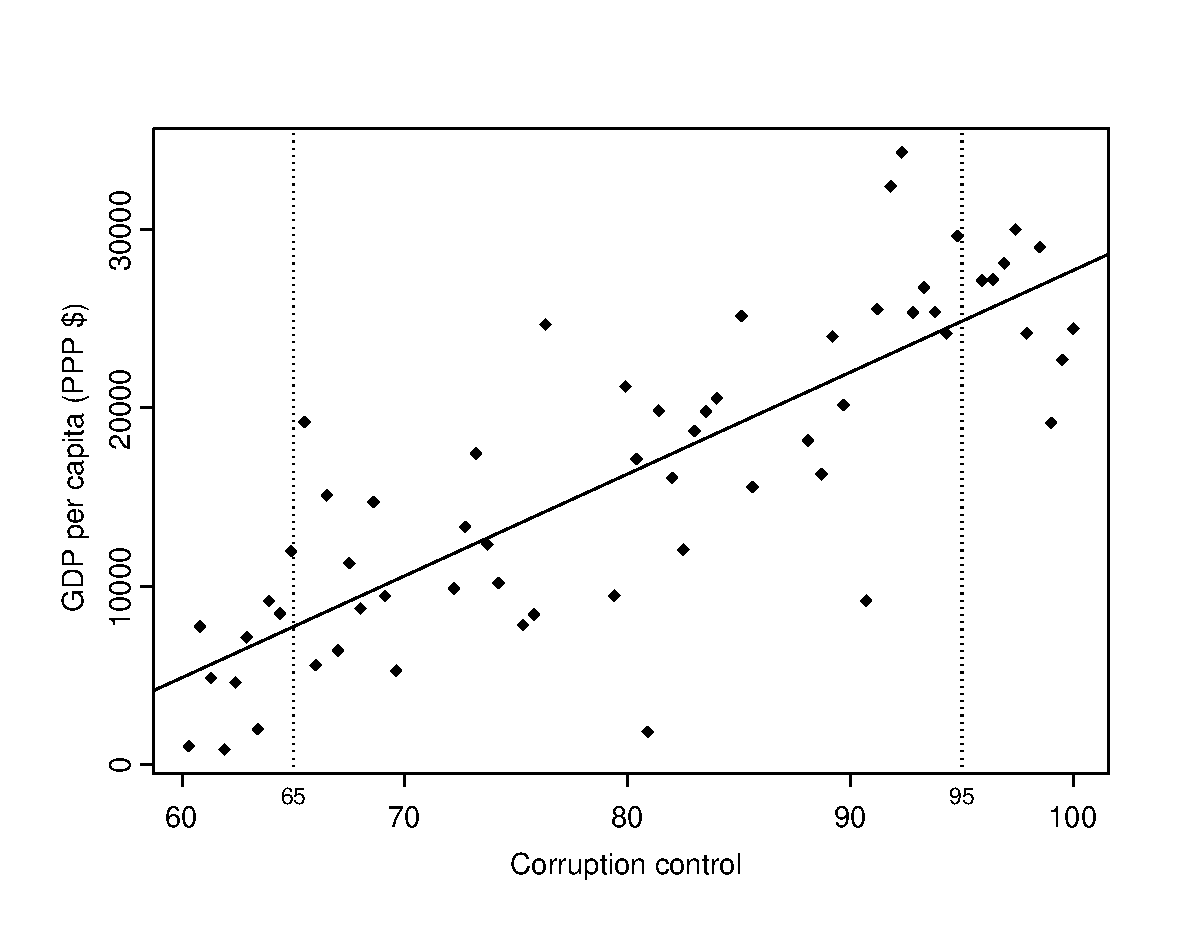
\includegraphics[width=13.5cm]{corruption2}

\end{figure}

Figure \ref{f_corruption2} shows the same scatterplot as Figure
\ref{f_corruption1}. Consider first one value of $X$ (Control of
corruption), say 65. To get a rough idea of the conditional distribution
of $Y$ (GDP per capita) given this value of $X$, we could examine the
sample distribution of the values of $Y$ for the units for which the
value of $X$ is close to 65. These correspond to the points near the
vertical line drawn at $X=65$ in Figure \ref{f_corruption2}. This can
be repeated for any value of $X$; for example, Figure
\ref{f_corruption2} also includes a vertical reference line at $X=95$,
for examining the conditional distribution of $Y$ given
$X=95$\footnote{This discussion is obviously rather approximate.
Strictly speaking, the conditional distribution of $Y$ given, say,
$X=65$ refers only to units with $X$ exactly rather than approximately
equal to 65. This, however, is difficult to illustrate using a sample,
because most values of a continuous $X$ appear at most once in a sample.
For reasons discussed later in this chapter, the present approximate
treatment still provides a reasonable general idea of the nature of the
kinds of associations considered here.}.

As in Chapter \ref{c_means}, associations between variables will here
be considered almost solely in terms of differences in the \emph{means} of
the conditional distributions of $Y$ at different values of $X$. For
example, Figure \ref{f_corruption2} suggests that the conditional mean
of $Y$ when X is 65 is around or just under 10000. At $X=95$, on the
other hand, the conditional mean seems to be between 20000 and 25000.
The mean of $Y$ is thus higher at the larger value of X. More generally,
this finding is consistent across the scatterplot, in that the
conditional mean of $Y$ appears to increase when we consider
increasingly large values of $X$, indicating that higher levels of
Control of corruption are associated with higher average levels of GDP.
This is often expressed by saying that the conditional mean of $Y$
increases when we ``increase'' $X$\footnote{This wording is
commonly used for convenience even in cases where the nature of $X$ is such that its
values can never actually be manipulated.}.
This is the sense in which we will examine associations
between continuous variables: does the conditional mean of $Y$ change
(increase or decrease) when we increase $X$? If it does, the two
variables are associated; if it does not, there is no association of
this kind. This definition also agrees with the one linking
association with prediction: if the mean of $Y$ is
different for different values of $X$, knowing the value of $X$ will
clearly help us in making predictions about likely values of $Y$. Based
on the information in Figure \ref{f_corruption2}, for example, our best
guesses of the GDPs of two countries would clearly be different if we
were told that the control of corruption measure was 65 for one country
and 95 for the other.

The \emph{nature} of the association between $X$ and $Y$ is
characterised by \emph{how} the values of $Y$ change when $X$ increases.
First, it is almost always reasonable to conceive these changes as
reasonably smooth and gradual. In other words, if two values of $X$ are
close to each other, the conditional means of $Y$ will be similar too;
for example, if the mean of $Y$ is 5 when $X=10$, its mean when
$X=10.01$ is likely to be quite close to 5 rather than, say, 405. In
technical terms, this means that the conditional mean of $Y$ will be
described by a smooth mathematical function of $X$. Graphically, the
means of $Y$ as $X$ increases will then trace a smooth curve in the
scatterplot. The simplest possibility for such a curve is a straight
line. This possibility is illustrated by plot (a) of Figure
\ref{f_scatterplots} (this and the other five plots in the figure
display artificial data, generated for this illustration). Here all of
the points fall on a line, so that when $X$ increases, the values of $Y$
increase at a constant rate. A relationship like this is known as a
\textbf{linear association} between $X$ and $Y$. Linear associations are
the starting point for examining associations between continuous
variables, and often the only ones considered. In this chapter we too
will focus almost completely on them.


\begin{figure}
\caption{
Scatterplots of artificial data sets of two variables. Each plot
also shows the best-fitting (least squares) straight line and the
correlation coefficient $r$.
}
\label{f_scatterplots}
%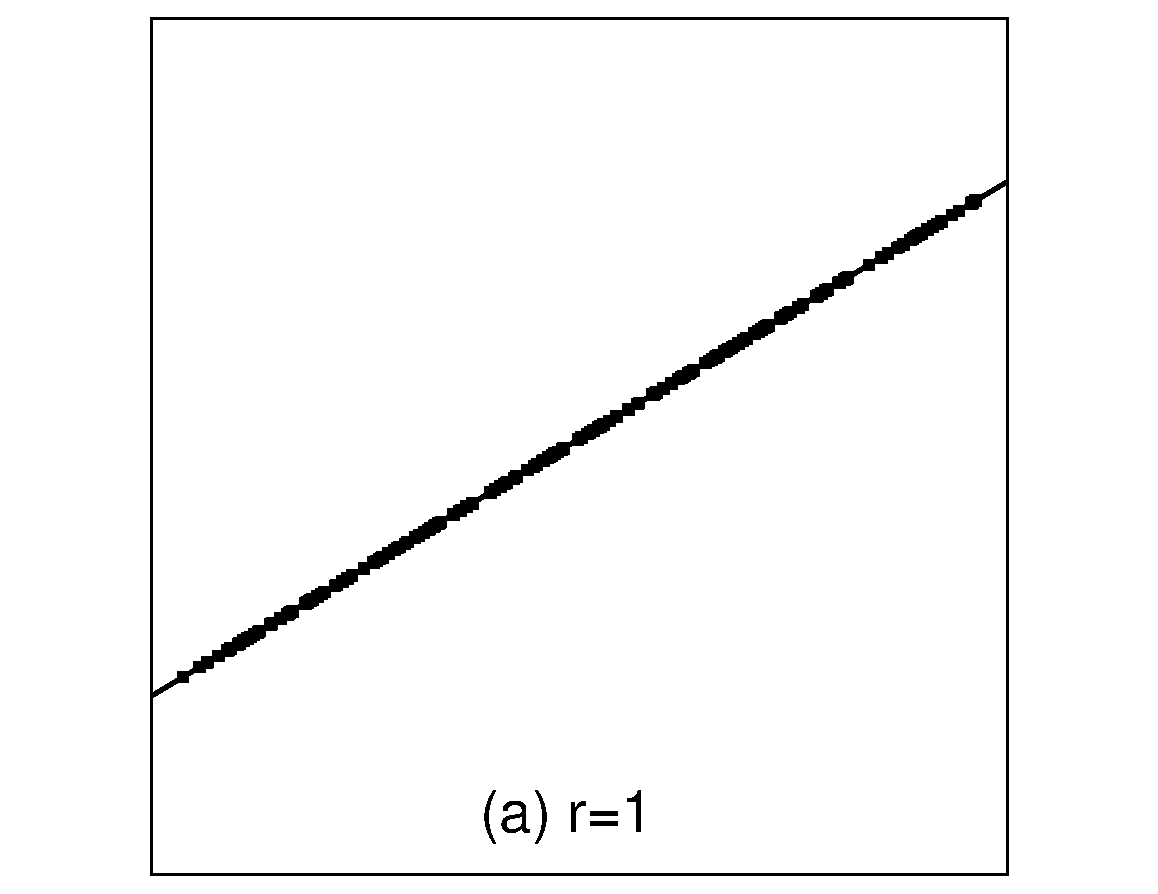
\includegraphics[width=12.5cm]{olspl1}
\begin{center}

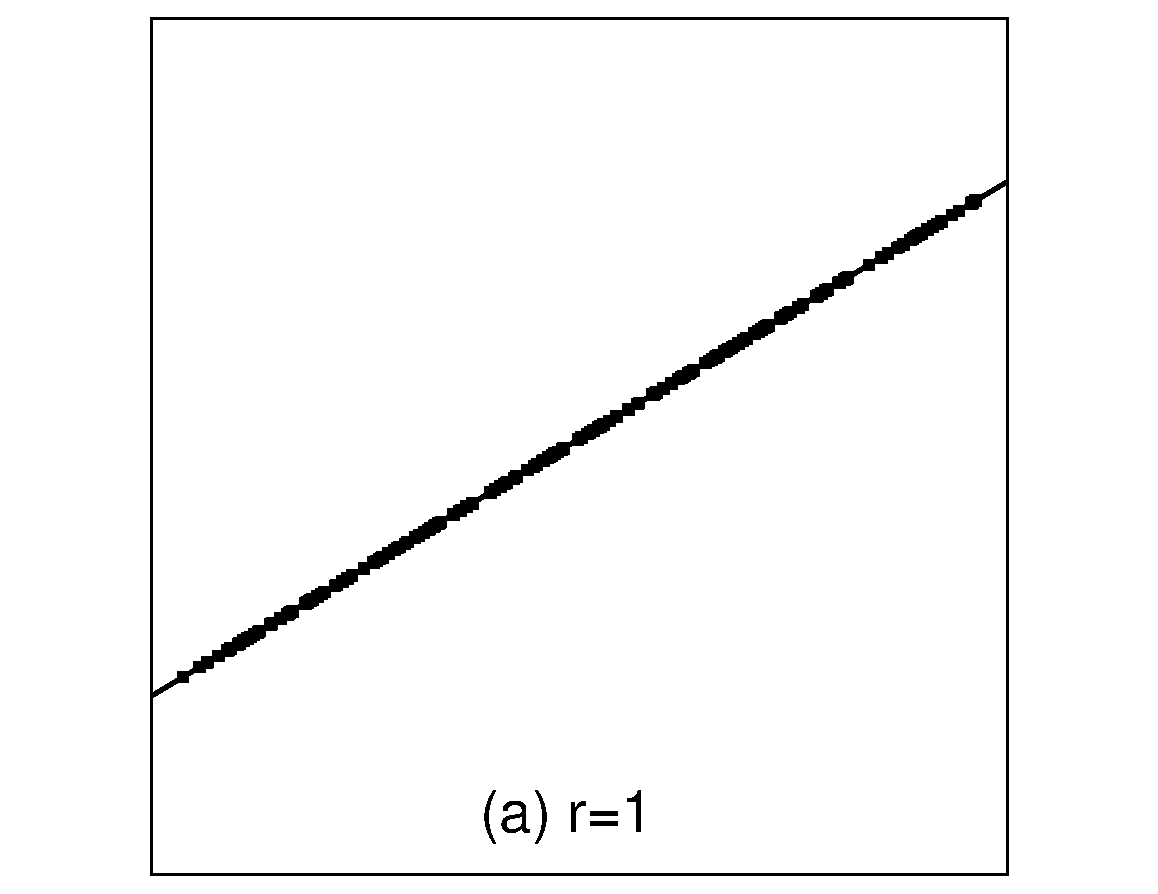
\includegraphics[width=8cm]{olspl1}
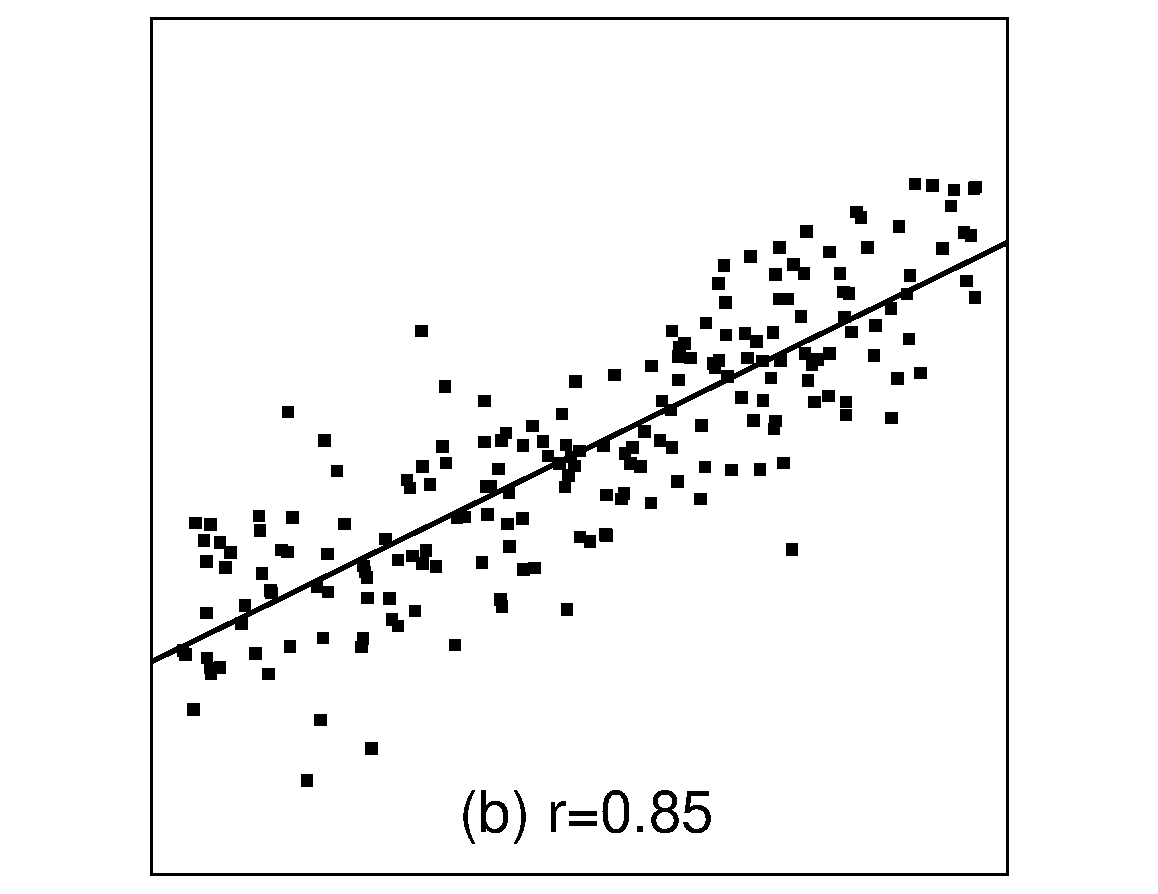
\includegraphics[width=8cm]{olspl2}\\


\includegraphics[width=8cm]{olspl3}
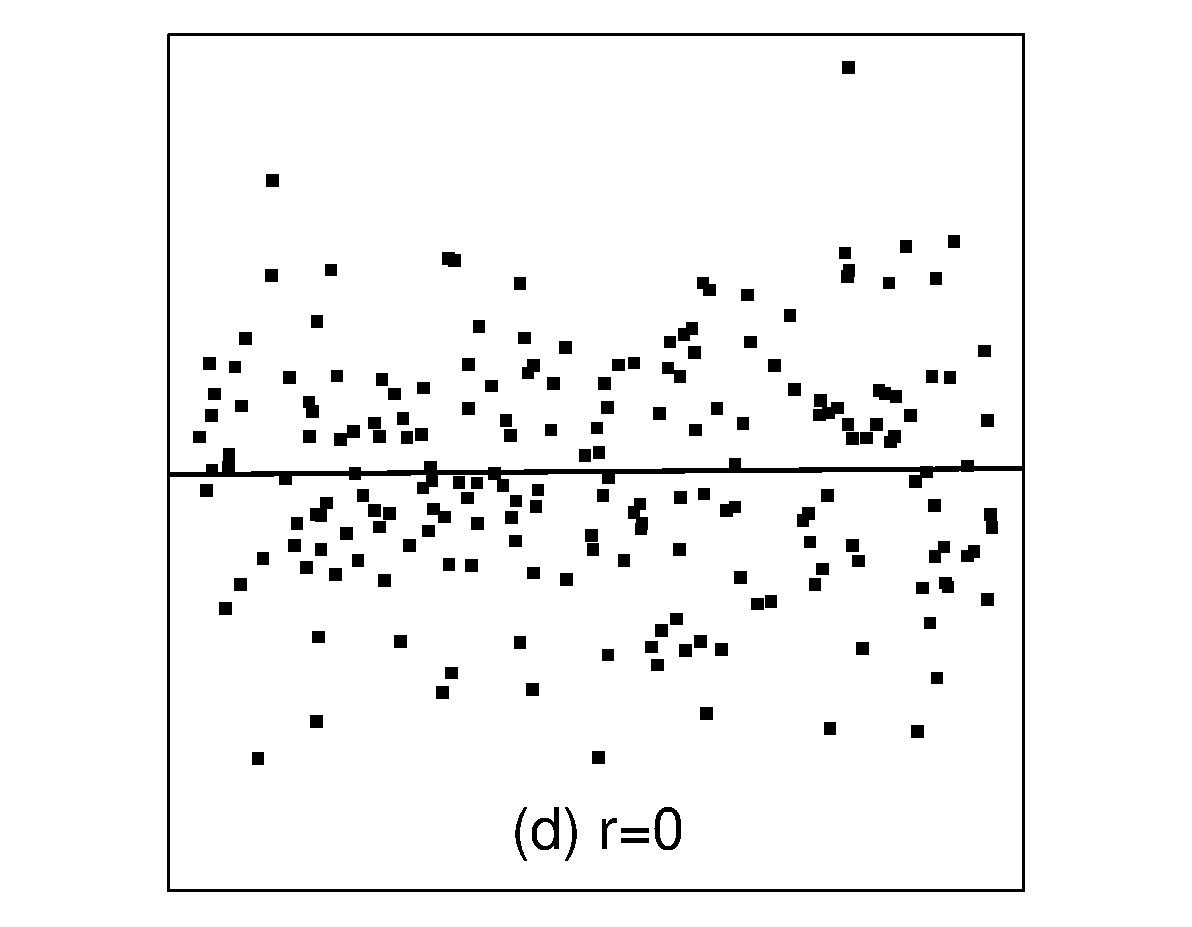
\includegraphics[width=8cm]{olspl4}\\

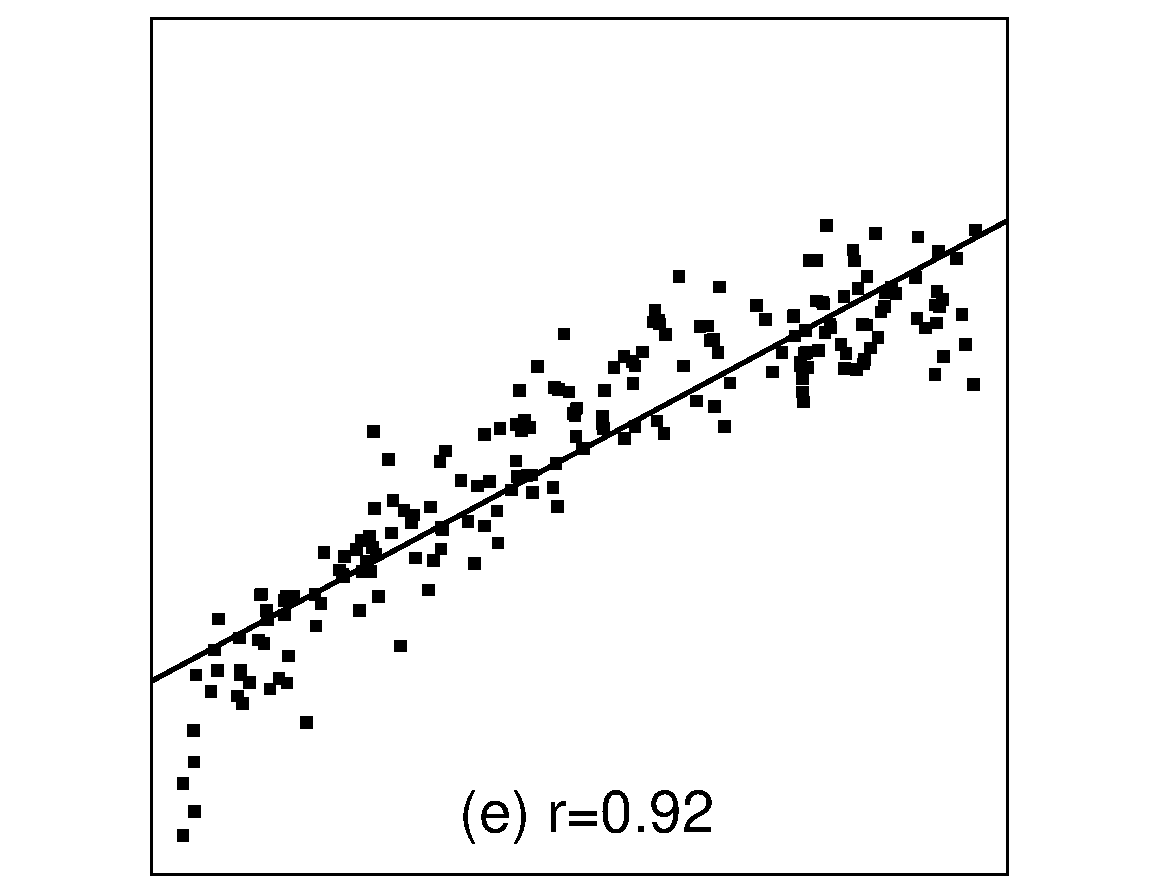
\includegraphics[width=8cm]{olspl5}
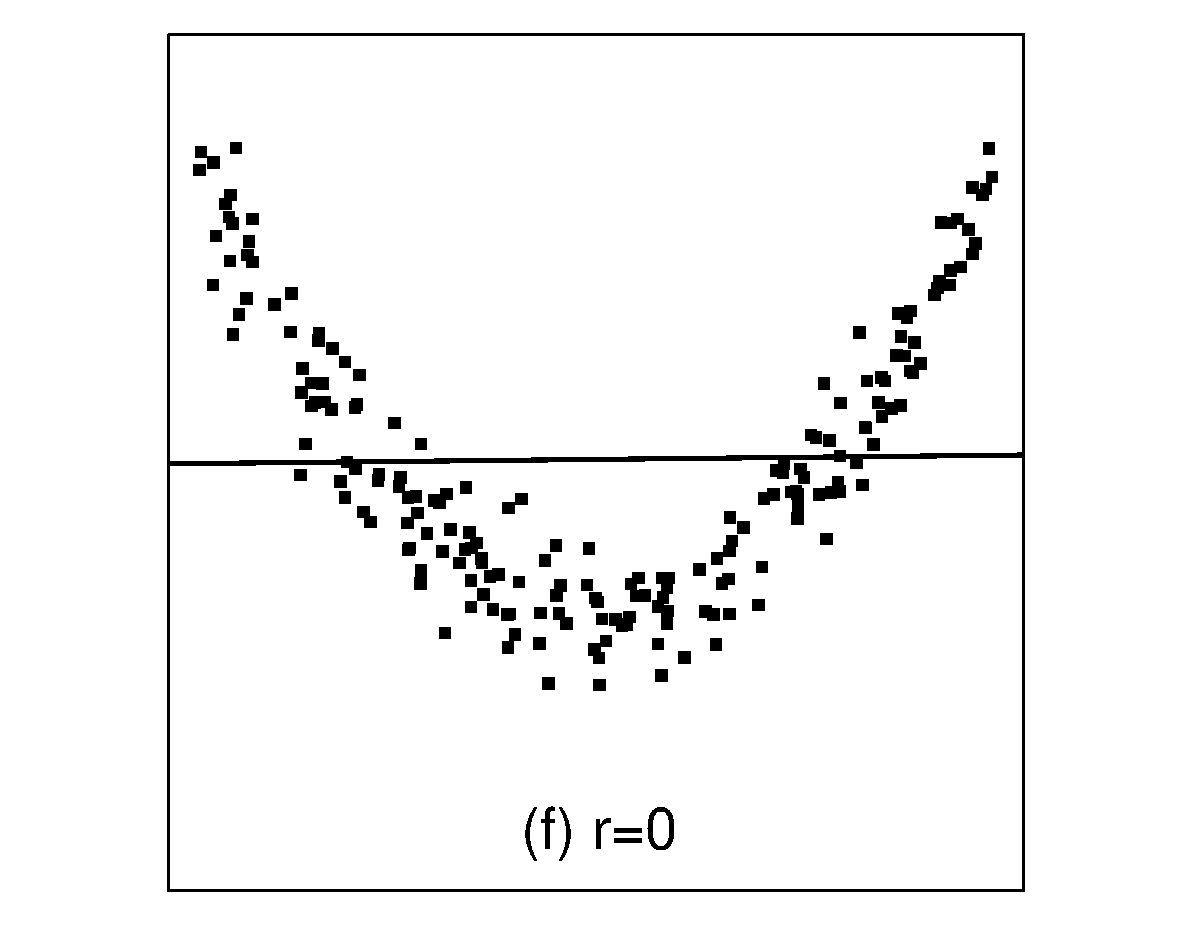
\includegraphics[width=8cm]{olspl6}\\
\end{center}
\end{figure}

In plot (a) of Figure \ref{f_scatterplots} all the points are exactly on
the straight line. This indicates a \emph{perfect} linear association,
where $Y$ can be predicted exactly if $X$ is known, so that the association is
\emph{deterministic}. Such a situation is neither realistic in
practice, nor necessary for the association to be
described as linear. All that is required for the latter is that the
conditional \emph{means} of $Y$ given different values of $X$ fall
(approximately) on a straight line. This is illustrated by plot (b) of
Figure \ref{f_scatterplots}, which shows a scatterplot of individual
observations together with an approximation of the line of the means of
$Y$ given $X$ (how the line was drawn will be explained later). Here the
linear association is not perfect, as the individual points are not all
on the same line but scattered around it. Nevertheless, the line seems
to capture an important systematic feature of the data, which is that
the \emph{average} values of $Y$ increase at an approximately constant
rate as $X$ increases. This combination of systematic and random
elements is characteristic of all statistical associations, and it is
also central to the formal setting for statistical inference for linear
associations described in Section \ref{s_regression_simple} below.

The \textbf{direction} of a linear association can be either
\textbf{positive} or \textbf{negative}. Plots (a) and (b) of Figure
\ref{f_scatterplots} show a positive association, because increasing $X$
is associated with increasing average values of $Y$. This is indicated
by the upward slope of the line describing the association. Plot (c)
shows an example of a negative association, where the line slopes
downwards and increasing values of $X$ are associated with decreasing
values of $Y$. The third possibility, illustrated by plot (d), is that
the line slopes neither up nor down, so that the mean of $Y$ is the same
for all values of $X$. In this case there is no (linear) association
between the variables.

Not all associations between continuous variables are linear, as shown
by the remaining two plots of Figure \ref{f_scatterplots}. These
illustrate two kinds of \textbf{nonlinear} associations. In plot (e),
the association is still clearly \emph{monotonic}, meaning that average
values of $Y$ change in the same direction --- here increase --- when
$X$ increases. The rate of this increase, however, is not constant, as
indicated by the slightly curved shape of the cloud of points. The
values of $Y$ seem to increase faster for small values of $X$ than for
large ones. A straight line drawn through the scatterplot captures the
general direction of the increase, but misses its nonlinearity. One
practical example of such a relationship is the one between years of
job experience and salary: it is often found that salary increases
fastest early on in a person's career and more slowly later on.

Plot (f) shows a nonlinear and nonmonotonic relationship: as $X$
increases, average values of $Y$ first decrease to a minimum, and then
increase again, resulting in a U-shaped scatterplot. A straight line is
clearly an entirely inadequate description of such a relationship. A
nonmonotonic association of this kind might be seen, for example, when
considering the dependence of the failure rates of some electrical
components ($Y$) on their age ($X$). It might then be that the failure
rates were high early (from quick failures of flawed components) and
late on (from inevitable wear and tear) and lowest in between for
``middle-aged but healthy'' components.

\begin{figure}[t]
\caption{A scatterplot of Control of corruption vs.\ GDP per capita for
163 countries in the Global Civil Society data set. The solid line is
the best-fitting (least squares) straight line for the points.}
\label{f_corruption3}

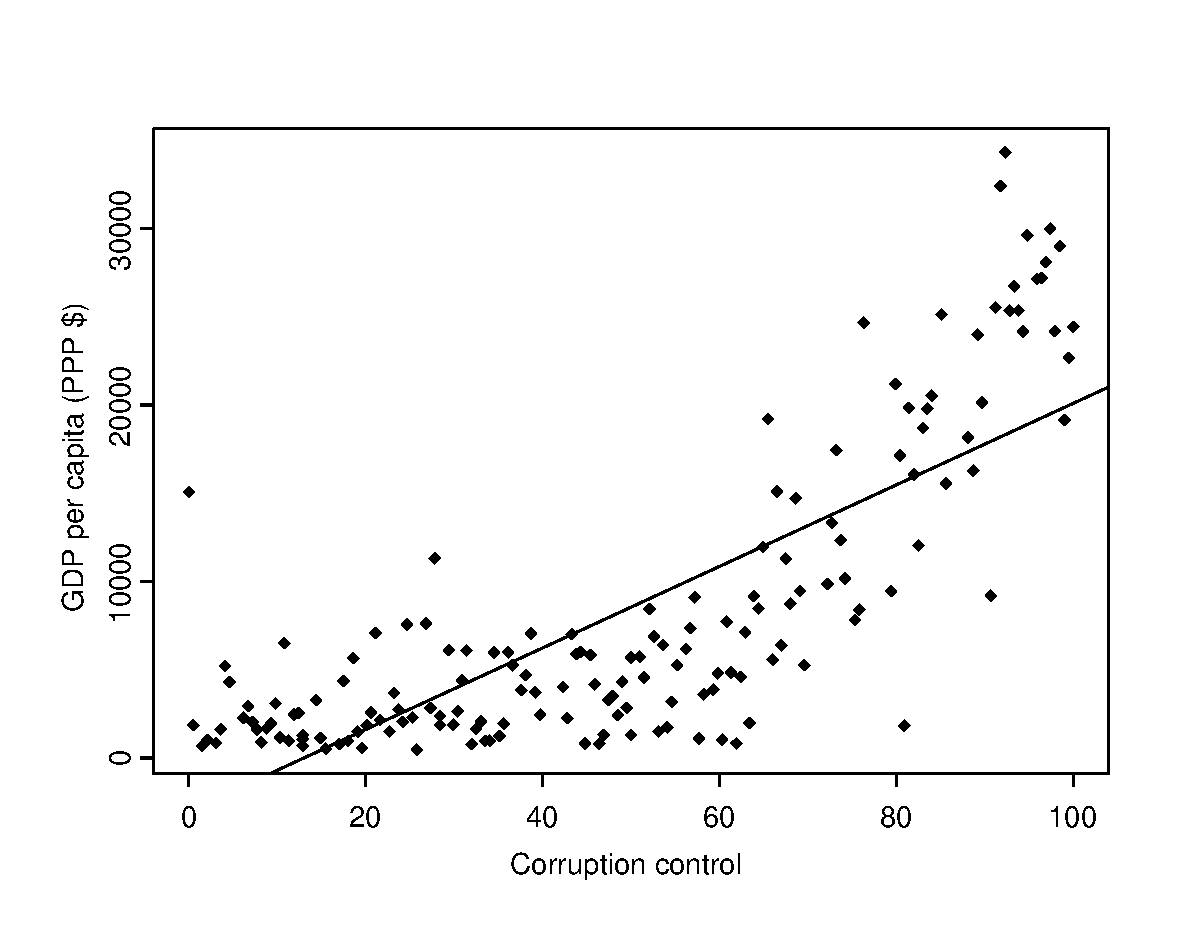
\includegraphics[width=13.5cm]{corruption3}

\end{figure}

Returning to real data, recall that we have so far considered control
of corruption and GDP per capita only among countries with a Control of
corruption score of at least 60. The scatterplot for these, shown in
Figure \ref{f_corruption2}, also includes a best-fitting straight line.
The observed relationship is clearly positive, and seems to be fairly
well described by a straight line. For countries with relatively low
levels of corruption, the association between control of corruption and GDP can
be reasonably well characterised as linear.

Consider now the set of all countries, including also those with
high levels of corruption (scores of less than 60). In a scatterplot for
them,  shown in Figure \ref{f_corruption3}, the points with at least 60
on the $X$-axis are the same as those in Figure \ref{f_corruption2}, and
the new points are to the left of them. The plot now shows a
nonlinear relationship comparable to the one in
plot (e) of Figure \ref{f_scatterplots}. The linear relationship which
was a good description for the countries considered above is thus not
adequate for the full set of countries. Instead, it seems that the
association is much weaker for the countries with high levels of
corruption, essentially all of which have fairly low values of GDP per
capita. The straight line fitted to the plot identifies the overall
positive association, but cannot describe its nonlinearity. This example
further illustrates how scatterplots can be used to examine
relationships between variables and to assess whether they can be best
described as linear or nonlinear associations\footnote{In this
particular example, a more closely linear association is obtained by
considering the logarithm of GDP as the response variable instead of GDP
itself. This approach, which is common in dealing with skewed variables
such as income, is, however, beyond the scope of this course.}.

So far we have said nothing about how the exact location and
direction of the straight lines shown in the figures have been selected.
These are determined so that the fitted line is in a certain
sense the best possible one for describing the data in the scatterplot.
Because the calculations needed for this are also (and more importantly)
used in the context of statistical inference for such
data, we will postpone a description of them until Section
\ref{ss_regression_simple_est}. For now we can treat the line simply as
a visual summary of the linear association in a scatterplot.

\subsection{Measures of association: covariance and correlation}
\label{ss_regression_descr_corr}

A scatterplot is a very powerful tool for examining sample associations
of pairs of variables in detail. Sometimes, however, this is more than
we really need for an initial summary of a data set, especially if there
are many variables and thus many possible pairs of them. It is then
convenient also to be able to summarise each pairwise association using
a single-number measure of association. This section introduces the
correlation coefficient, the most common such measure for continuous
variables. It is a measure of the strength of \emph{linear} associations
of the kind defined above.

Suppose that we consider two variables, denoted $X$ and $Y$. This again
implies a distinction between an explanatory and a response variable, to
maintain continuity of notation between different parts of this chapter.
The correlation coefficient itself, however, is completely symmetric, so
that its value for a pair of variables will be the same whether or not
we treat one or the other of them as explanatory for the other.
First, recall from equation (\ref{sd}) that the sample standard
deviations of the two variables are calculated as
\begin{equation}
s_{x} = \sqrt{\frac{\sum(X_{i}-\bar{X})^{2}}{n-1}}
\text{and}
s_{y} = \sqrt{\frac{\sum (Y_{i}-\bar{Y})^{2}}{n-1}}
\label{sdyx}
\end{equation}
where the subscripts $x$ and $y$ identify the two variables, and
$\bar{X}$ and $\bar{Y}$ are their sample means. A new statistic
is the
\textbf{sample covariance} between $X$ and $Y$, defined as
\begin{equation}
s_{xy} = \frac{\sum (X_{i}-\bar{X})(Y_{i}-\bar{Y})}{n-1}.
\label{sxy}
\end{equation}
This is a measure of linear association between $X$ and $Y$. It is
positive if the sample association is positive and negative if the
association is negative.

In theoretical statistics, covariance is the fundamental summary of
sample and population associations between two continuous variables. For
descriptive purposes, however, it has the inconvenient feature that its
magnitude depends on the units in which $X$ and $Y$ are measured. This
makes it difficult to judge whether a value of the covariance
for particular variables should be regarded as large or small. To remove
this complication, we can standardise the sample covariance by dividing
it by the standard deviations, to obtain the statistic
\begin{equation}
r=\frac{s_{xy}}{s_{x}s_{y}} =
\frac
{
\sum (X_{i}-\bar{X})(Y_{i}-\bar{Y})
}{
\sqrt{
\sum\left(X_{i}-\bar{X}\right)^{2}
\sum\left(Y_{i}-\bar{Y}\right)^{2}}
}.
\label{corr}
\end{equation}
This is the (sample) \textbf{correlation} coefficient, or correlation
for short, between $X$ and $Y$. It is also often (e.g.\ in SPSS) known as
\emph{Pearson's} correlation coefficient after Karl Pearson (of the
$\chi^{2}$ test, see page \pageref{p_pearson}), although both the word and the statistic
are really due to Sir Francis Galton\footnote{ Galton, F.\ (1888).
``Co-relations and their measurement, chiefly from anthropometric
data''. \emph{Proceedings of the Royal Society of London}, \textbf{45},
135--145.}.

The properties of the correlation coefficient can be described by going
through the same list as for the $\gamma$ coefficient in Section
\ref{ss_descr1_2cat_gamma}. While doing so, it is useful to refer to
the examples in Figure \ref{f_scatterplots}, where the correlations are
also shown.
\begin{itemize}
\item
\textbf{Sign}: Correlation is positive if the \emph{linear} association
between the variables is positive, i.e.\ if the best-fitting straight
line slopes upwards (as in plots a, b and e) and negative if the
association is negative (c). A zero correlation indicates complete lack
of linear association (d and f).
\item
\textbf{Extreme values}: The largest possible correlation is $+1$
(plot a) and the smallest $-1$, indicating perfect positive and negative
linear associations respectively. More generally, the magnitude of the
correlation indicates the strength of the association, so that the
closer to $+1$ or $-1$ the correlation is, the stronger the association
(e.g.\ compare plots a--d). It should again be noted that the
correlation captures only the linear aspect of the association, as
illustrated by the two nonlinear cases in Figure \ref{f_scatterplots}.
In plot (e), there is curvature but also a strong positive trend, and
the latter is reflected in a fairly high correlation. In plot (f), the
trend is absent and the correlation is 0, even though there is an
obvious nonlinear relationship. Thus the correlation coefficient is a
reasonable initial summary of the strength of association in (e), but
completely misleading in (f).
\item
\textbf{Formal interpretation}: The correlation coefficient cannot be
interpreted as a Proportional Reduction in Error (PRE) measure, but its
square can. The latter statistic, so-called coefficient of determination
or $R^{2}$, is described in Section \ref{ss_regression_simple_int}.
\item
\textbf{Substantive interpretation}: As with any measure of association,
the question of whether a particular sample correlation is high
or low is not a purely statistical question, but depends on the nature
of the variables. This can be judged properly only with the help of
experience of correlations between similar variables in different
contexts. As one very rough rule thumb it might be said that in many
social science contexts correlations greater than 0.4 (or smaller than
$-0.4$) would typically be considered noteworthy and ones greater than 0.7
quite strong.
\end{itemize}

Returning to real data, Table \ref{t_civilsoc_r} shows the correlation
coefficients for all fifteen distinct pairs of the six continuous
variables in the Global Civil Society data set mentioned on page
\pageref{p_civilsoc}. This is an example of a \textbf{correlation
matrix}, which is simply a table with the variables as both its rows and
columns, and the correlation between each pair of variables given at the
intersection of corresponding row and column. For example, the
correlation of GDP per capita and School enrolment is here 0.42. This is
shown at the intersection of the first row (GDP) and fifth column
(School enrolment), and also of the fifth row and first column. In
general, every correlation is shown twice in the matrix, once in its
upper triangle and once in the lower. The triangles are separated by a
list of ones on the diagonal of the matrix. This simply indicates that
the correlation of any variable with itself is 1, which is true by
definition and thus of no real interest.

\begin{table}
\caption{
Correlation matrix of six continuous variables in the Global Civil
Society data set. See page \pageref{p_civilsoc} for more information on the
variables.}
\label{t_civilsoc_r}
\begin{center}
\begin{tabular}{|r|rrrrrr|}\hline
& \multicolumn{6}{|c|}{Variable} \\
Variable & GDP & Gini & Pol.\ & Corrupt.\ & School & IMR \\ \hline
GDP per capita [GDP] & 1 & -0.39 & 0.51 & 0.77 & 0.42 & -0.62 \\
Income inequality [Gini] & -0.39 & 1& -0.15 & -0.27 & -0.27 & 0.42 \\
Political rights [Pol.] & 0.51 & -0.15 & 1& 0.59 & 0.40 & -0.44 \\
Control of corruption [Corrupt.]& 0.77 & -0.27 & 0.59 & 1& 0.41 & -0.64 \\
School enrolment [School] & 0.42 & -0.27 & 0.40 & 0.41 &1 & -0.73 \\
Infant mortality [IMR] & -0.62 & 0.42 & -0.44 & -0.64 & -0.73 & 1\\
\hline
\end{tabular}
\end{center}
\end{table}

All of the observed associations in this example are in unsurprising
directions. For example, School enrolment is positively correlated with
GDP, Political rights and Control of corruption, and negatively
correlated with Income inequality and Infant mortality. In other words,
countries with large percentages of children enrolled in primary school
tend to have high levels of GDP per capita and of political rights and
civil liberties,  and low levels of corruption, income inequality and
infant mortality. The strongest associations in these data are
between GDP per capita and Control of corruption ($r=0.77$) and School
enrolment and Infant mortality rate ($r=-0.73$), and the weakest between
Income inequality on the one hand and Political rights, Control of
corruption and School enrolment on the other (correlations of $-0.15$,
$-0.27$ and $-0.27$ respectively).

These correlations describe only
the linear element of sample associations, but give no
hint of any nonlinear ones. For example, the correlation of 0.77
between GDP and Control of corruption
summarises the way the observations
cluster around the straight line shown in
Figure \ref{f_corruption3}. The correlation is
high because this increase in GDP as Control of corruption increases is
quite strong, but it gives no indication of the nonlinearity of the
association. A scatterplot is needed for revealing
this feature of the data. The correlation for the restricted set of
countries shown in Figure \ref{f_corruption2} is 0.82.

A correlation coefficient can also be defined for the joint population
distribution of two variables. The sample correlation $r$ can then be
treated as an estimate of the population correlation, which is often
denoted by $\rho$ (the lower-case Greek ``rho''). Statistical inference
for the population correlation can also be derived. For example, SPSS
automatically outputs significance tests for the null hypothesis that
$\rho$ is 0, i.e.\ that there is no linear association between $X$ and
$Y$ in the population. Here, however, we will not discuss this, choosing
to treat $r$ purely as a descriptive sample statistic.
The next section provides a different set of tools for
inference on population associations.

\section{Simple linear regression models}
\label{s_regression_simple}

\subsection{Introduction}
\label{ss_regression_simple_intro}

The rest of this course is devoted to the method of linear regression
modelling. Its
purpose is the analysis of associations in cases where the response
variable is a continuous, interval level variable, and the
possibly several explanatory variables can be of any type. We begin
in this section with \emph{simple} linear regression, where
there is only one explanatory variable. We will further assume that this
is also continuous. The situation considered here is thus the same as in
the previous section, but here the focus will be on statistical
inference rather than description. Most of the main concepts of linear
regression can be introduced in this context. Those that go beyond it
are described in subsequent sections. Section \ref{s_regression_multiple}
introduces \emph{multiple} regression involving more than
one explanatory variable. The use of categorical explanatory variables
in such models is explained in Section \ref{s_regression_dummies}. Finally,
Section \ref{s_regression_rest} gives a brief review of some further
aspects of linear regression modelling which are not covered on this
course.

\newpage
\emph{Example: Predictors of Infant Mortality Rate}

The concepts of linear regression models will be illustrated as they are
introduced with a second example from the Global Civil Society data set.
The response variable will now be Infant Mortality Rate (IMR). This is
an illuminating outcome variable, because it is a sensitive and
unquestionably important reflection of a country's wellbeing; whatever
we mean by ``development'', it is difficult to disagree that high levels
of it should coincide with low levels of infant mortality. We will
initially consider only one explanatory variable, Net primary school
enrolment ratio, referred to as ``School enrolment'' for short. This is
defined as the percentage of all children of primary school age who are
enrolled in school. Enrolment numbers and the population size are
often obtained from different official sources, which sometimes leads to
discrepancies. In particular, School enrolment for several countries is
recorded as over 100, which is logically impossible. This is an
illustration of the kinds of measurement errors often affecting
variables in the social sciences. We will use the School enrolment
values as recorded, even though they are known to contain some error.

A scatterplot of IMR vs.\ School enrolment is shown in Figure
\ref{f_imr1}, together with the best-fitting straight line. Later
we will also consider three additional explanatory variables:
Control of corruption, Income inequality and Income level of the country
in three categories (c.f.\ page \pageref{p_civilsoc}). For further
reference, Table \ref{t_imrvars} shows various summary statistics for
these variables. Throughout, the analyses are restricted to those 111
countries for which all of the five variables are recorded. For this
reason the correlations in Table \ref{t_imrvars} differ slightly from
those in Table \ref{t_civilsoc_r}, where each correlation was calculated
for all the countries with non-missing values of that pair of
variables.


\begin{figure}[t]
\caption{A scatterplot of net primary school enrolment ratio vs.\
Infant mortality rate for countries
in the Global Civil Society data set ($n=111$). The solid line is
the best-fitting (least squares) straight line for the points.}
\label{f_imr1}

\begin{center}
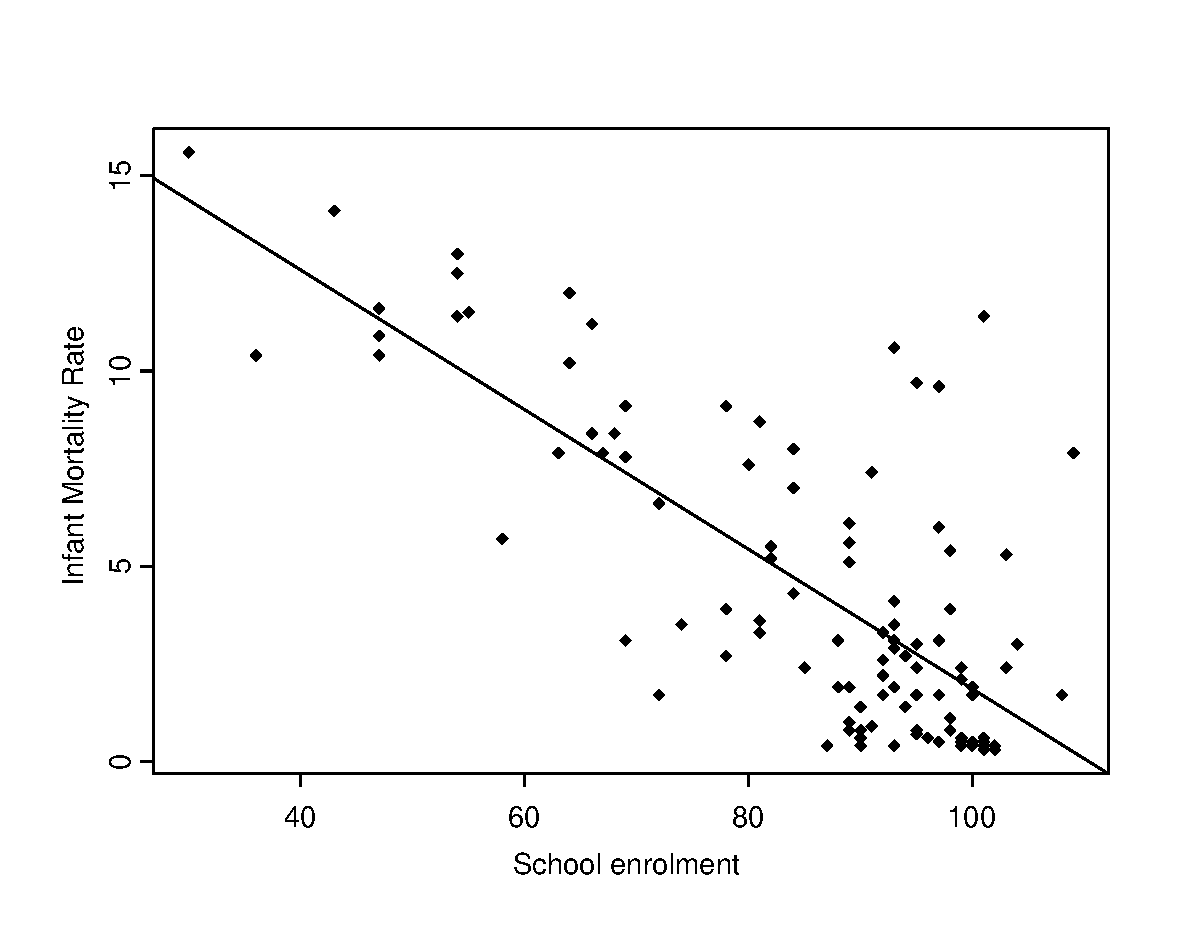
\includegraphics[width=13.5cm]{imr1}
\end{center}

\end{figure}

\begin{table}
\caption{Summary statistics for Infant Mortality Rate (IMR) and
explanatory variables for it considered in the examples of Sections
\ref{s_regression_simple} and \ref{s_regression_multiple} ($n=111$). See
page \pageref{p_civilsoc} for further information on the variables.}
\label{t_imrvars}
\begin{center}
\begin{tabular}{|lrrrr|}\hline
& \multicolumn{4}{c|}{Variable} \\
& & School & Control of & Income \\
& IMR & enrolment & corruption & inequality  \\ \hline
\multicolumn{5}{l}{\emph{Summary statistics}} \\ \hline
Mean & 4.3 & 86.1 & 50.1 & 40.5 \\
std.\ deviation & 4.0 & 16.7 & 28.4 & 10.2 \\
Minimum & 0.3 & 30.0 & 3.6 & 24.4\\
Maximum & 15.6 & 109.0 & 100.0 & 70.7 \\ \hline
\multicolumn{5}{l}{\emph{Correlation matrix}} \\ \hline
IMR & 1& -0.75 & -0.60 & 0.39 \\
School enrolment & -0.75 & 1 & 0.39 & -0.27 \\
Control of corruption & -0.60 & 0.39 & 1& -0.27 \\
Income inequality & 0.39 & -0.27 & -0.27 & 1\\ \hline
\multicolumn{5}{l}{\emph{Means for countries in different income
categories}} \\ \hline
Low income ($n=41$)& 8.2& 72.1& 27.5 & 41.7\\
Middle income ($n=48$)& 2.8& 92.5& 50.8& 43.3\\
High income ($n=22$)& 0.5& 98.4& 90.7 & 32.0\\
\hline
\end{tabular}
\end{center}
\end{table}

\subsection{Definition of the model}
\label{ss_regression_simple_def}

The simple linear regression model defined in this section is a
statistical model for a continuous, interval level response
variable $Y$ given a single explanatory variable $X$, such as
IMR given School enrolment. The model will be used to carry out
statistical inference on the association between the variables in a
population (which in the IMR example is clearly again of the conceptual
variety).

For motivation, recall first the situation considered in Section
\ref{s_means_inference}. There the data consisted of observations $(Y_{i},
X_{i})$ for $i=1,2,\dots,n$, which were assumed to be statistically
independent. The response variable $Y$ was continuous but $X$ had only
two possible values, coded 1 and 2. A model was then set up where the
population distribution of $Y$ had mean $\mu_{1}$ and variance
$\sigma^{2}_{1}$ for units with $X=1$, and mean $\mu_{2}$ and variance
$\sigma^{2}_{2}$ when $X=2$. In some cases it was further assumed that
the population distributions were both normal, and that the population
variances were equal, i.e.\ that $\sigma^{2}_{1}=\sigma^{2}_{2}$, with
their common value denoted $\sigma^{2}$. With these further assumptions,
which will also be used here, the model for $Y$ given a dichotomous $X$
stated that (1) observations for different units $i$ were statistically
independent; (2) each $Y_{i}$ was sampled at random from a population
distribution which was normal with mean $\mu_{i}$ and variance
$\sigma^{2}$; and (3) $\mu_{i}$ depended on $X_{i}$ so that it was equal
to $\mu_{1}$ if $X_{i}$ was 1 and $\mu_{2}$ if $X_{i}$ was 2.

The situation in this section is exactly the same, except that $X$ is
now continuous instead of dichotomous. We will use the same basic
model, but will change the specification of the conditional mean
$\mu_{i}$ appropriately. In the light of the discussion in previous
sections of this chapter, it is no surprise that this will be defined in
such a way that it describes a linear association between $X$ and $Y$.
This is done by setting $\mu_{i}=\alpha+\beta X_{i}$, where $\alpha$ and
$\beta$ are unknown population parameters. This is the equation of
straight line (we will return to it
in the next section). With this specification, the model for observations
$(Y_{1},X_{1}), (Y_{2}, X_{2}), \dots, (Y_{n}, X_{n})$ becomes
\begin{enumerate}
\item
Observations for different units $i$ ($=1,2,\dots,n$) are statistically
independent.
\item
Each $Y_{i}$ is normally distributed with mean $\mu_{i}$ and variance
$\sigma^{2}$.
\item
The means $\mu_{i}$ depend on $X_{i}$ through $\mu_{i}=\alpha+\beta
X_{i}$.
\end{enumerate}
Often the model is expressed in an equivalent form where 2.\ and 3.\ are
combined as
\begin{equation}
Y_{i}=\alpha+\beta X_{i} +\epsilon_{i}
\label{slinmodel}
\end{equation}
where each $\epsilon_{i}$ is normally distributed with mean 0 and
variance $\sigma^{2}$. The $\epsilon_{i}$ are known as \textbf{error
terms} or \textbf{population residuals} (and the letter $\epsilon$ is
the lower-case Greek ``epsilon''). This formulation of the model clearly
separates the mean of $Y_{i}$, which traces the straight line
$\alpha+\beta X_{i}$ as $X_{i}$ changes, from the variation around that
line, which is described by the variability of $\epsilon_{i}$.

The model defined above is known as the \textbf{simple linear regression
model}:
\begin{itemize}
\item
\textbf{Simple} because it has only one explanatory variable, as
opposed to \emph{multiple} linear regression models
which will have more than one.
\item
\textbf{Linear} because it specifies a linear
association between $X$ and $Y$.\footnote{This is slightly misleading: what actually matters in general
is that the conditional mean is a linear function of the
\emph{parameters} $\alpha$ and $\beta$. This need not concern us at this
stage.}
\item
\textbf{Regression}: This is now an established part of the name
of the model, although the origins of the word
are not central to the use of the model\footnote{Galton, F.\ (1886). ``Regression towards mediocrity in
hereditary stature''. \emph{Journal of the Anthropological Institute},
\textbf{15}, 246--263. The original context is essentially the
one discussed on courses on research
design as ``regression toward the mean''.}.
\item
\textbf{Model}, because this is a statistical model in the sense
discussed on page \pageref{p_model}. In other
words, the model is always only a simplified abstraction of the true,
immeasurably complex processes which determine the values of $Y$.
Nevertheless, it is believed that a well-chosen model can be useful for
explaining and predicting observed values of $Y$. This spirit is
captured by the well-known statement by
the statistician George Box\footnote{This exact phrase apparently first
appears in Box, G.E.P.\ (1979). Robustness in the strategy of scientific
model building. In Launer, R.L.\ and Wilkinson, G.N., \emph{Robustness
in Statistics}, pp.\ 201--236.}:
\begin{quote}
\emph{All models are wrong, but some are useful.}
\end{quote}
A model like this has the advantage that it reduces the examination of
associations in the population to estimation and inference on a small
number of model parameters, in the case of the
simple linear regression model just $\alpha$, $\beta$ and $\sigma^{2}$.
\end{itemize}
Of course, not all models are equally appropriate for given data, and
some will be both wrong and useless. The results from a model should
thus be seriously presented and interpreted only if the model is deemed
to be reasonably adequate. For the simple linear regression model, this
can be partly done by examining whether the scatterplot between $X$ and
$Y$ appears to be reasonably consistent with a linear relationship. Some
further comments on the assessment of model adequacy will be given in
Section \ref{s_regression_rest}.

\subsection{Interpretation of the model parameters}
\label{ss_regression_simple_int}

The simple linear regression model (\ref{slinmodel}) has three
parameters, $\alpha$, $\beta$ and $\sigma^{2}$. Each of these has its
own interpretation, which are explained in this section. Sometimes it
will be useful to illustrate the definition with specific numerical
values, for which we will use ones for the model for IMR
given School enrolment in our example. SPSS output for this model is
shown in Figure \ref{f_spss_linreg}. Note that although these values are
first used here to illustrate the interpretation of the \emph{population}
parameters in the model, they are of course only estimates (of a
kind explained in the next section) of those parameters. Other parts of
the SPSS output will be explained later in this chapter.

\begin{figure}[t]
\caption{SPSS output for a simple linear regression model for Infant
mortality rate given School enrolment in the Global Civil Society data.}
\label{f_spss_linreg}

%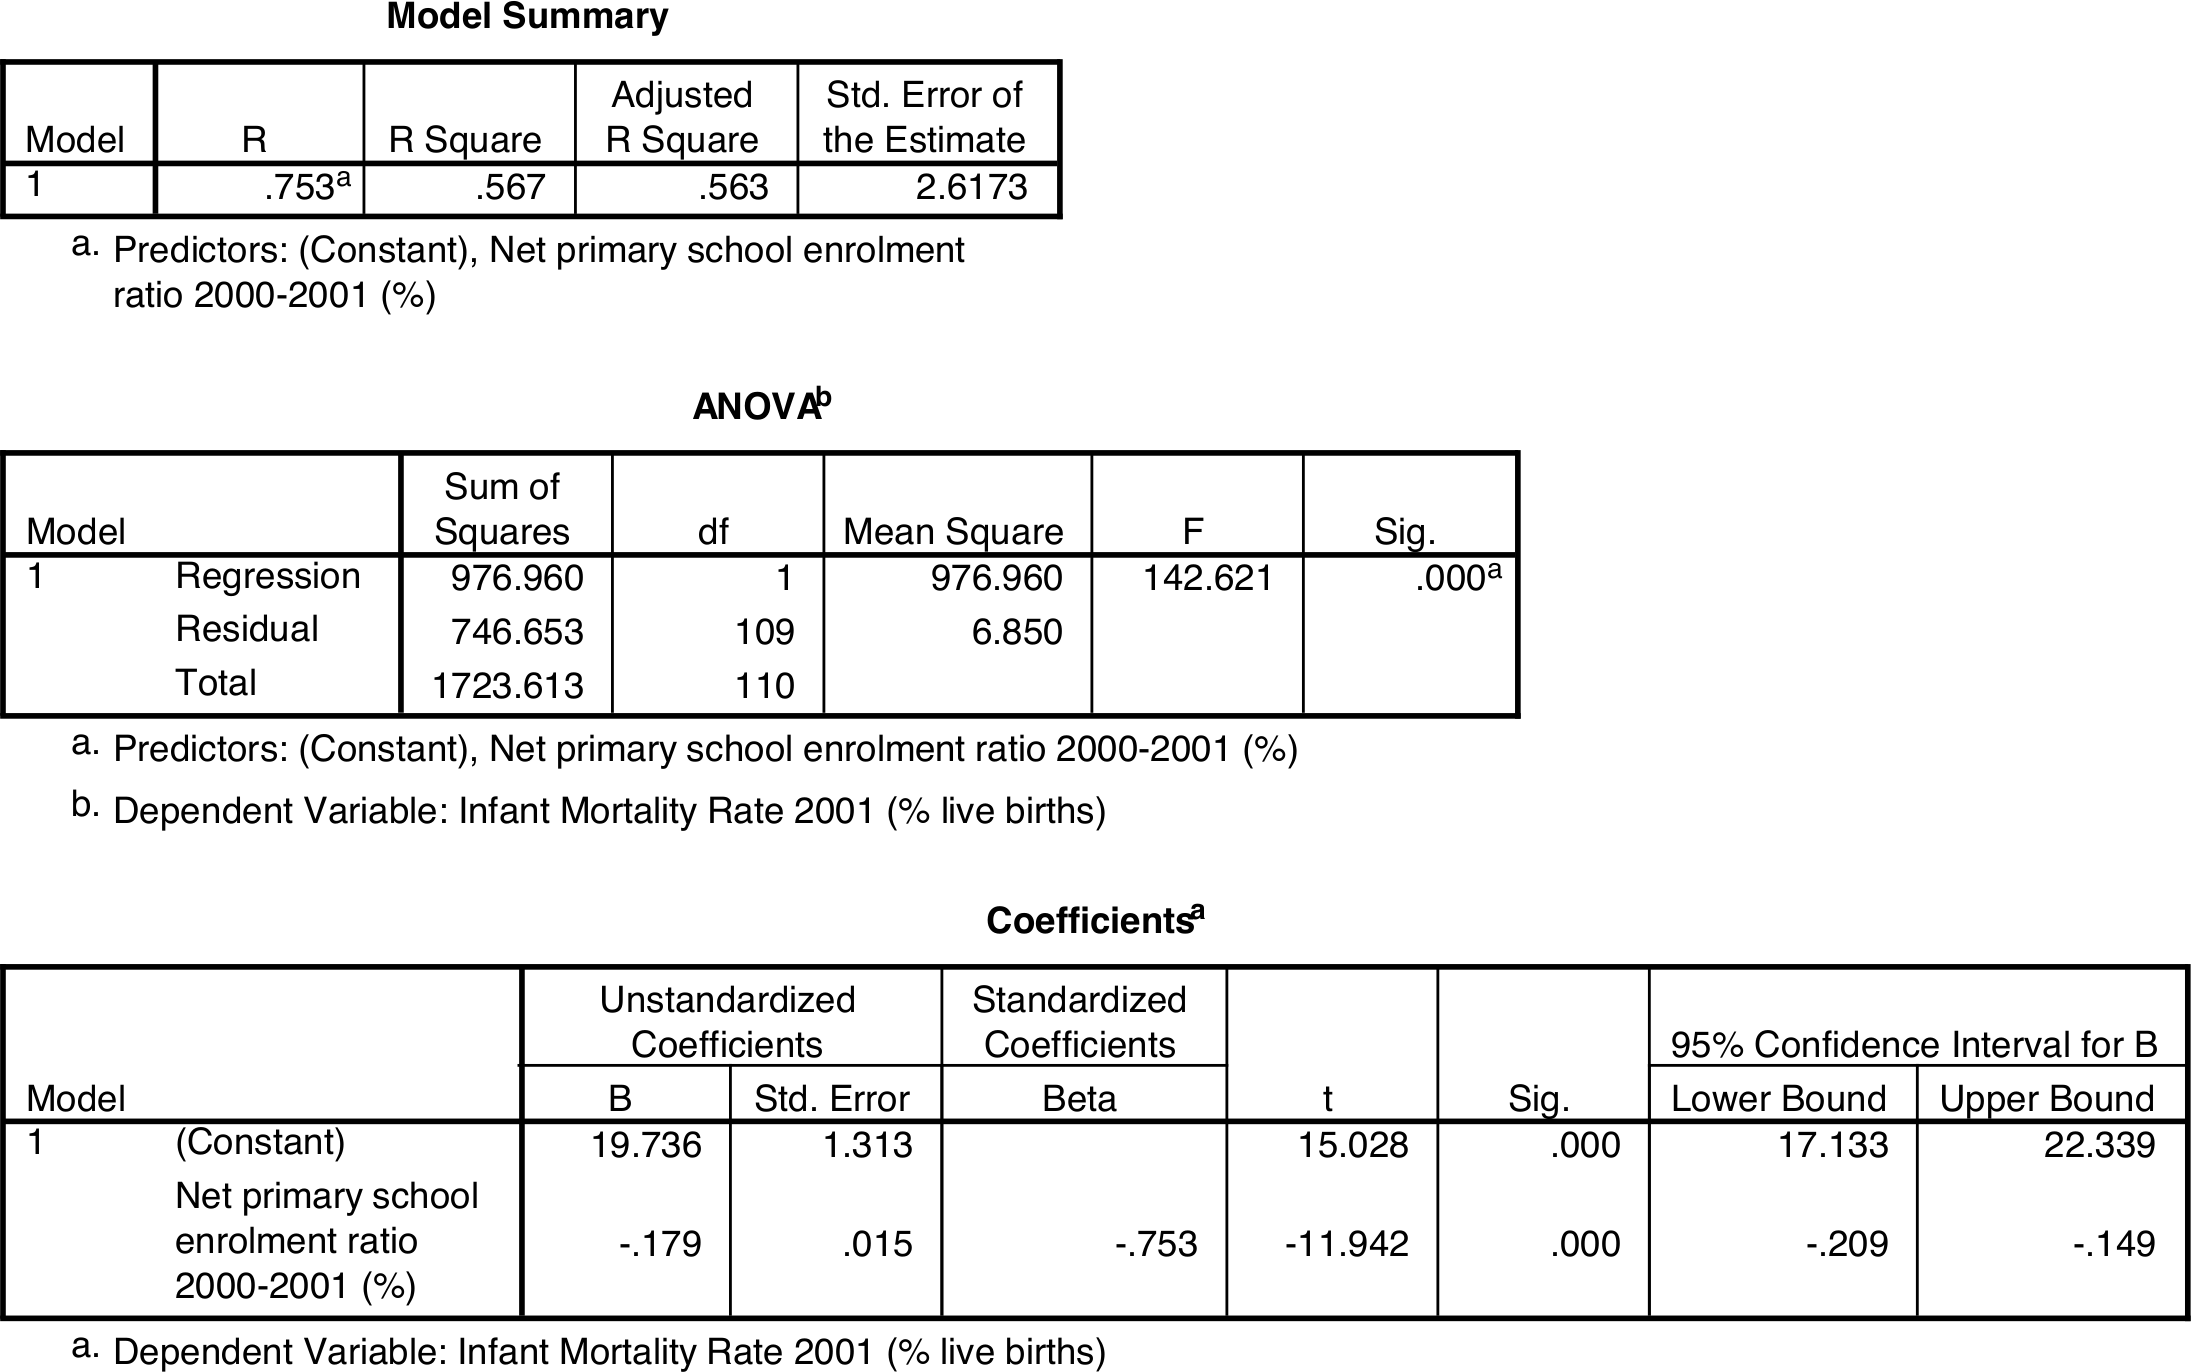
\includegraphics[bb=100 370 500 750, width=140mm]{spsslinreg}
%\includegraphics[bb=100 370 500 750, angle=-90, width=140mm]{spsslinreg2}
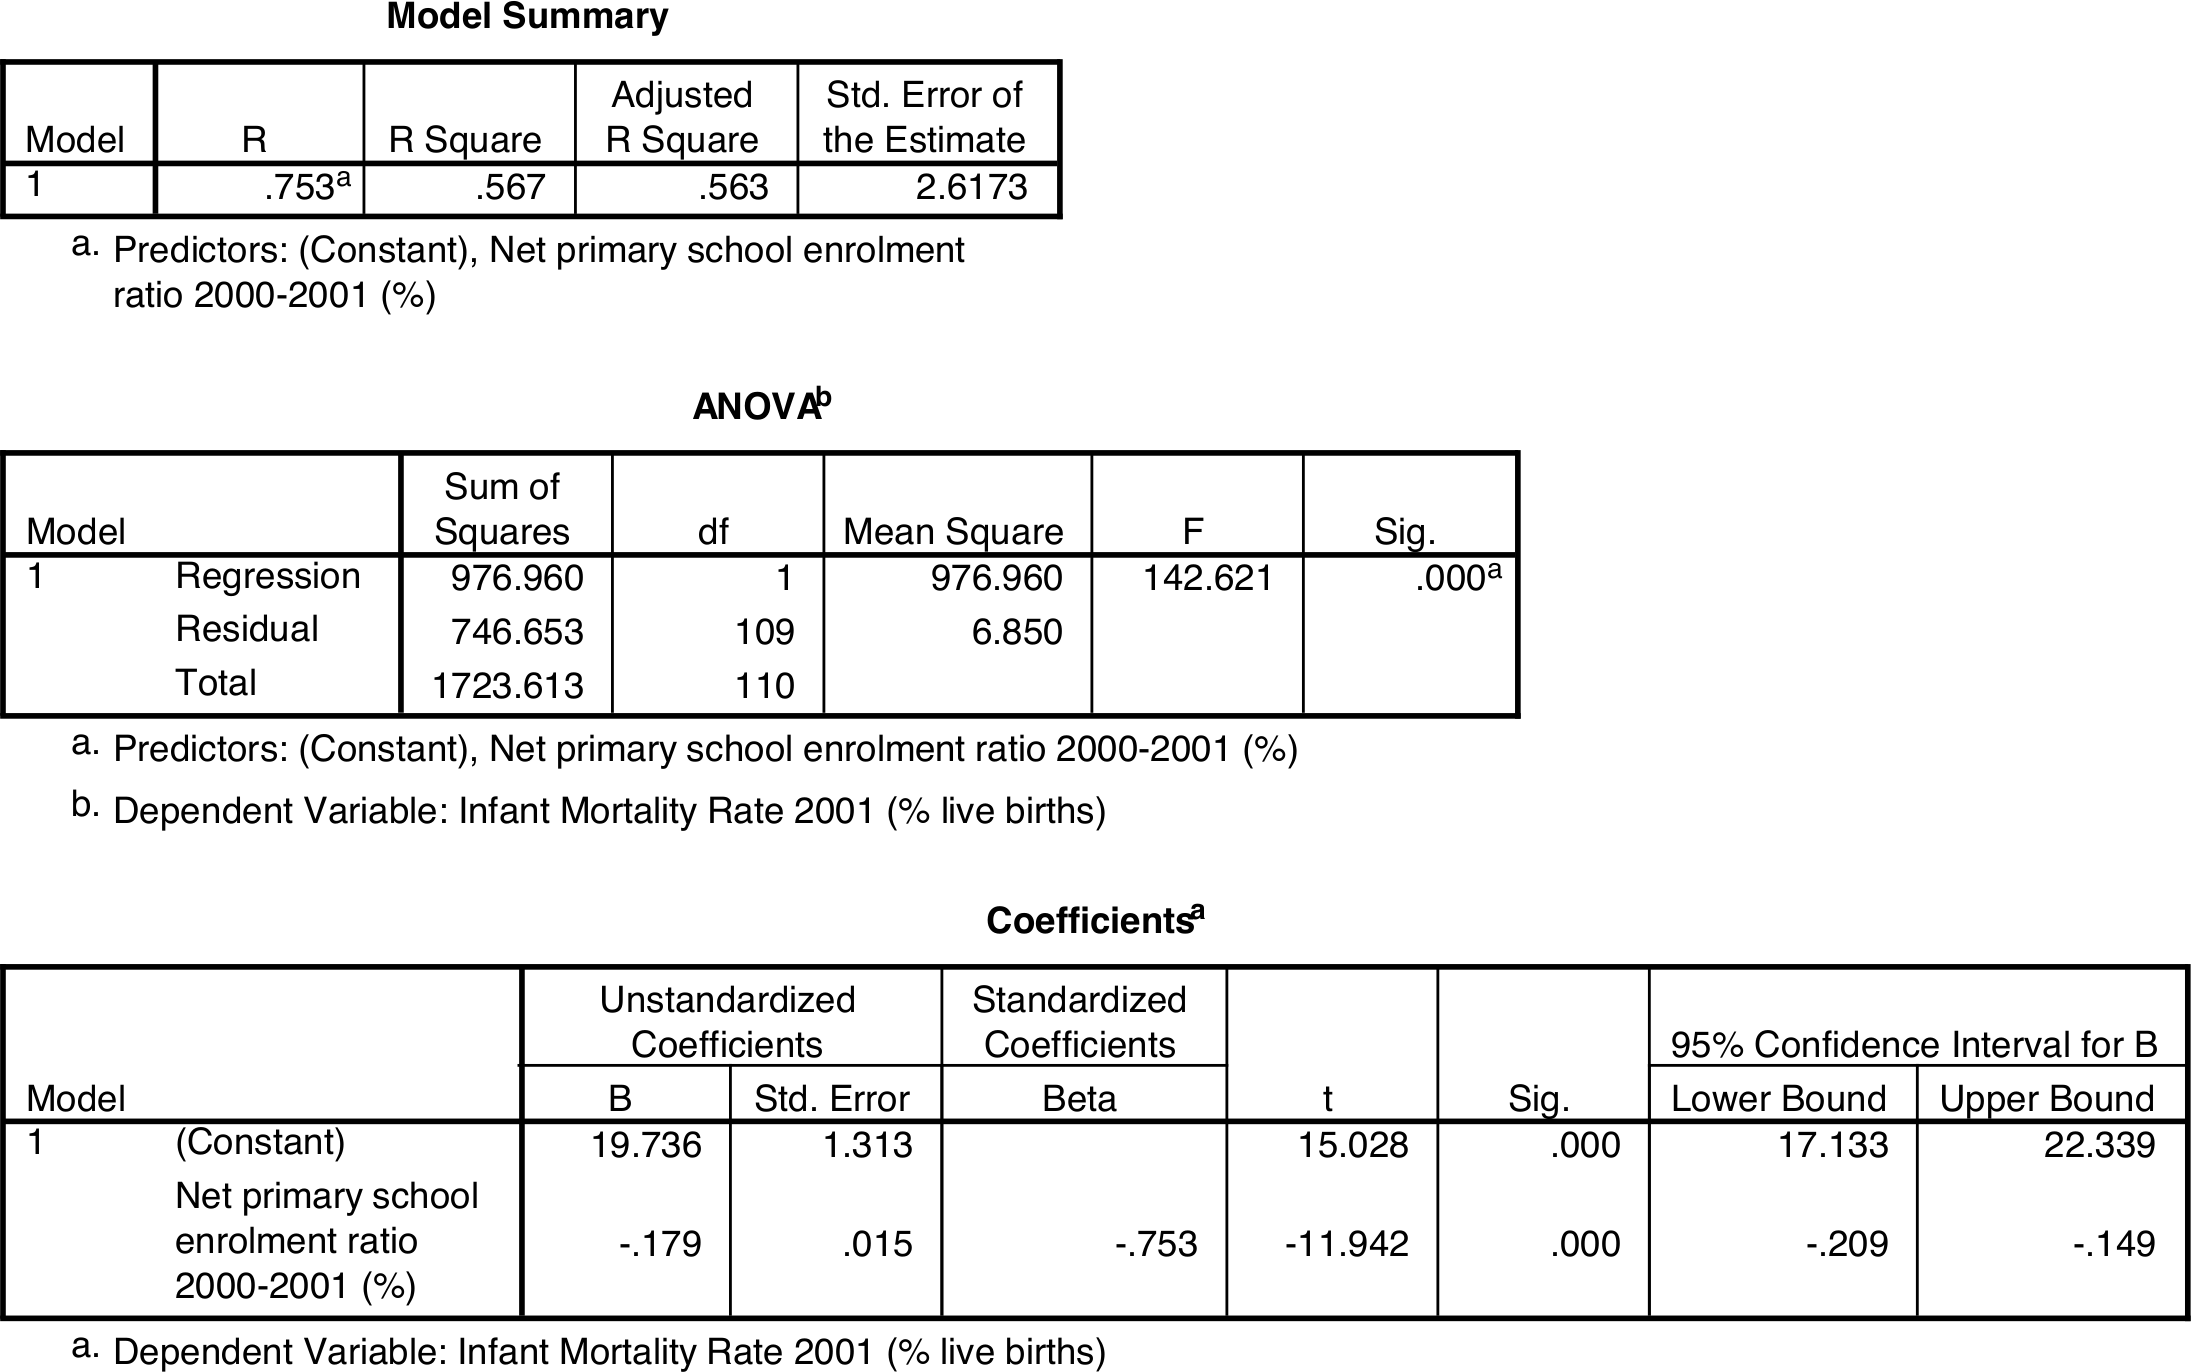
\includegraphics[bb=100 90 470 590, angle=-90, width=144mm]{spsslinreg}

\end{figure}

According to the model, the conditional mean (also often known as the
conditional \textbf{expected value})
of $Y$ given $X$ in the
population is (dropping the subscript $i$ for now for notational
simplicity) $\mu=\alpha+\beta X$. The two parameters $\alpha$ and
$\beta$ in this formula are known as \textbf{regression coefficients}.
They are interpreted as follows:
\begin{itemize}
\item
$\alpha$ is the expected value of $Y$ when $X$ is equal to 0. It is
known as the \textbf{intercept} or \textbf{constant} term of the model.
\item
$\beta$ is the change in the expected value of $Y$ when $X$ increases by
1 unit. It is known as the \textbf{slope} term or the
\textbf{coefficient of} $X$.
\end{itemize}
Just to include one mathematical proof in this coursepack,
these results can be derived as follows:
\begin{itemize}
\item
When $X=0$, the mean of $Y$ is $\mu=\alpha+\beta X=\alpha+\beta\times 0
=\alpha+0=\alpha$.
\item
Compare two observations, one with value $X$ of the explanatory
variable, and the other with one unit more, i.e.\ $X+1$. The
corresponding means of $Y$ are


\begin{tabular}{rlll}
with $X+1$: & $\mu$ &
$=\alpha+\beta\times (X+1)$ &
$=\alpha+\beta X +\beta$ \\
with $X$: & $\mu$ &
& $=\alpha+\beta X$ \\ \hline
Difference: & & & $\beta$
\end{tabular}
\end{itemize}
which completes the proof of the claims above --- Q.E.D. In case you
prefer a graphical summary, this is given in Figure \ref{f_linmod_params}.

\begin{figure}
\caption{Illustration of the interpretation of the regression
coefficients of a simple linear regression model.}
\label{f_linmod_params}

\begin{center}

\includegraphics[width=12.5cm]{lmparams}
\end{center}

\end{figure}

The most important parameter of the model, and usually the only one
really discussed in interpreting the results, is $\beta$, the regression
coefficient of $X$. It is also called the slope because it is literally
the slope of the regression line, as shown in Figure
\ref{f_linmod_params}. It is the only parameter in the model which
describes the association between $X$ and $Y$, and it does so in the
above terms of expected changes in $Y$ corresponding to changes in X
($\beta$ is also related to the correlation between $X$ and $Y$, in a
way explained in the next section). The sign of $\beta$ indicates the
direction of the association. When $\beta$ is positive (greater than 0),
the regression line slopes upwards and increasing $X$ thus also
increases the expected value of $Y$ --- in other words, the association
between $X$ and $Y$ is positive. This is the case illustrated in Figure
\ref{f_linmod_params}. If $\beta$ is negative, the regression line
slopes downwards and the association is also negative. Finally, if
$\beta$ is zero, the line is parallel with the $X$-axis, so that
changing $X$ does not change the expected value of $Y$. Thus
$\beta=0$ corresponds to no (linear) association between $X$ and $Y$.

In the real example shown in Figure \ref{f_spss_linreg}, $X$ is School
enrolment and $Y$ is IMR. In SPSS output, the
estimated regression coefficients are given in the
``\textbf{Coefficients}'' table in the column labelled ``B'' under
``Unstandardized coefficients''. The estimated constant
term $\alpha$ is given in the row labelled ``(Constant)'', and the slope
term on the next row, labelled  with the name or label of the
explanatory variable as specified in the SPSS data file --- here ``Net
primary school enrolment ratio 2000-2001 (\%)''.  The value of the
intercept is here 19.736 and the slope coefficient is $-0.179$. The
estimated regression line for expected IMR is thus $19.736-0.179 X$,
where $X$ denotes School enrolment. This is the line shown in
Figure \ref{f_imr1}.

Because the slope coefficient in the example is negative, the
association between the variables is also negative, i.e.\ higher levels
of school enrolment are associated with lower levels of infant
mortality. More specifically, every increase of one unit (here one
percentage point) in School enrolment is associated with a decrease of
0.179 units (here percentage points) in expected IMR.

Since the meaning of $\beta$ is related to a unit increase of the
explanatory variable, the interpretation of its magnitude depends on
what those units are. In many cases one unit of $X$ is too small or too
large for convenient interpretation. For example, a change of one
percentage point in School enrolment is rather small, given that the
range of this variable in our data is 79 percentage points (c.f.\ Table
\ref{t_imrvars}). In such cases the results can easily be reexpressed by
using multiples of $\beta$: specifically, the effect on expected value
of $Y$ of changing $X$ by $A$ units is obtained by multiplying $\beta$
by $A$. For instance, in our example the estimated effect of increasing
School enrolment by 10 percentage points is to decrease expected IMR by
$10\times 0.179=1.79$ percentage points.

The constant term $\alpha$ is a necessary part of the model, but it is
almost never of interest in itself. This is because the expected value
of $Y$ at $X=0$ is rarely specifically interesting. Very often $X=0$ is
also unrealistic, as in our example where it corresponds to a country
with zero primary school enrolment. There are fortunately no such
countries in the data, where the lowest School enrolment is 30\%. It is
then of no interest to discuss expected IMR for a hypothetical country
where no children went to school. Doing so would also represent
unwarranted \emph{extrapolation} of the model beyond the range of the
observed data. Even though the estimated linear model seems to fit
reasonably well for these data, this is no guarantee that it would do so
also for countries with much lower school enrolment, even if they
existed.

The third parameter of the simple regression model is $\sigma^{2}$. This
is the variance of the conditional distribution of $Y$ given $X$. It is
also known as the \textbf{conditional variance} of $Y$, the
\textbf{error variance} or the \textbf{residual variance}. Similarly,
its square root $\sigma$ is known as the conditional, error or
\textbf{residual standard deviation}. To understand $\sigma$, let us
consider a single value of $X$, such as one corresponding to one of the
vertical dashed lines in Figure \ref{f_linmod_params} or, say, school
enrolment of 85 in Figure \ref{f_imr1}. The model specifies a
distribution for $Y$ given any such value of $X$. If we were to
(hypothetically) collect a large number of observations, all with this
same value of $X$, the distribution of $Y$ for them would describe the
conditional distribution of $Y$ given that value of $X$. The model
states that the average of these values, i.e.\ the conditional mean of
$Y$, is $\alpha+\beta X$, which is the point on the regression line
corresponding to $X$. The individual values of $Y$, however, would of
course not all be on the line but somewhere around it, some above and
some below.

The linear regression model further specifies that the form of the
conditional distribution of $Y$ is approximately normal. You can try to
visualise this by imagining a normal probability curve (c.f.\ Figure
\ref{f_norm1}) on the vertical line from $X$, centered on the regression
line and sticking up from the page. The bell shape of the curve
indicates that most of the values of $Y$ for a given $X$ will be close
to the regression line, and only small proportions of them far from it.
The residual standard deviation $\sigma$ is the standard deviation of
this conditional normal distribution, in essence describing how tightly
concentrated values of $Y$ tend to be around the regression line. The
model assumes, mainly for simplicity, that the same value of
$\sigma$ applies to the conditional distributions at all values of $X$;
this is known as the assumption of \emph{homoscedasticity}.

In SPSS output, an estimate of $\sigma$ is given in the ``\textbf{Model
Summary}'' table under the misleading label ``Std.\ Error of the
Estimate''.
An estimate of the residual variance $\sigma^{2}$ is found also in the
``\textbf{ANOVA}'' table under ``Mean Square'' for ``Residual''. In our
example the estimate of $\sigma$ is 2.6173 (and that of $\sigma^{2}$ is
6.85). This is usually not of direct interest for interpretation,
but it will be a necessary component of some parts of the
analysis discussed below.

\subsection{Estimation of the parameters}
\label{ss_regression_simple_est}

Since the regression coefficients $\alpha$ and $\beta$ and the residual
standard deviation $\sigma$ are unknown population parameters, we will
need to use the observed data to obtain sensible estimates for them. How
to do so is now less obvious than in the cases of simple means and
proportions considered before. This section explains the standard method
of estimation for the parameters of linear regression models.

We will denote estimates of $\alpha$ and $\beta$ by $\hat{\alpha}$ and
$\hat{\beta}$ (``alpha-hat'' and ``beta-hat'') respectively (other
notations are also often used, e.g.\ $a$ and $b$). Similarly, we can
define %the quantities
\[
\hat{Y}=\hat{\alpha}+\hat{\beta} X
\]
for $Y$ given any value of $X$. These are the values on the estimated
regression line. They are known as \textbf{fitted values} for $Y$, and
estimating the parameters of the regression model is often referred to
as ``fitting the model'' to the observed data. The fitted values
represent our predictions of expected values of $Y$ given $X$, so they
are also known as \textbf{predicted values} of $Y$.

In particular, fitted values $\hat{Y}_{i}=\hat{\alpha}+\hat{\beta}X_{i}$
can be calculated at the values $X_{i}$ of the explanatory variable
$X$ for each unit $i$ in the observed sample. These can then be compared
to the correponding values $Y_{i}$ of the response variable. Their
differences $Y_{i}-\hat{Y}_{i}$ are known as the (sample) \textbf{residuals}.
These quantities are illustrated in Figure \ref{f_residuals}. This shows
a fitted regression line, which is in fact the one for IMR
given School enrolment also shown in Figure \ref{f_imr1}. Also shown are
two points $(X_{i}, Y_{i})$. These are also from Figure
\ref{f_imr1}; the rest have been omitted to simplify the plot. The point
further to the left is the one for Mali, which has School enrolment
$X_{i}=43.0$ and IMR $Y_{i}=14.1$. Using the estimated
coefficients $\hat{\alpha}=19.736$ and $\hat{\beta}=-0.179$ in Figure
\ref{f_spss_linreg}, the fitted value for Mali is
$\hat{Y}_{i}=19.736-0.179\times 43.0=12.0$. Their difference is the
residual $Y_{i}-\hat{Y}_{i}=14.1-12.0=2.1$. Because the observed value
is here larger than the fitted value, the residual is positive and the
observed value is above the fitted line, as shown in Figure
\ref{f_residuals}.

\begin{figure}
\caption{Illustration of the quantities involved in the definitions of
least squares estimates and the coefficient of determination $R^{2}$.
See the text for explanation.}
\label{f_residuals}
\begin{center}

\includegraphics[width=13.5cm]{lmresids}
\end{center}
$Y_{i}-\hat{Y}_{i}$

$Y_{i}-\hat{Y}_{i}$

$\bar{Y}$

$\hat{Y}_{i}-\bar{Y}$

$Y_{i}-\bar{Y}$

$\hat{Y}=\hat{\alpha}+\hat{\beta} X$
\end{figure}

The second point shown in Figure \ref{f_residuals} corresponds to the
observation for Ghana, for which $X_{i}=58.0$ and $Y_{i}=5.7$. The
fitted value is then $\hat{Y}_{i}=19.736-0.179\times 58.0=9.4$ and the
residual $Y_{i}-\hat{Y}_{i}=5.7-9.4=-3.7$. Because the observed value is
now smaller than the fitted value, the residual is negative and the
observed $Y_{i}$ is below the fitted regression line.

So far we have still not explained how the specific values of the
parameter estimates in Figure \ref{f_spss_linreg} were obtained. In
doing so, we are faced with the task of identifying a regression line
which provides the best fit to the observed points in a scatterplot like
Figure \ref{f_imr1}. Each possible choice of $\hat{\alpha}$ and
$\hat{\beta}$ corresponds to a different regression line, and some
choices are clearly better than others. For example, it seems
intuitively obvious that it would be better for the line to go through
the cloud of points rather than stay completely outside it. To make such
considerations explicit, the residuals can be used as a criterion of
model fit. The aim will then be to make the total magnitude of the
residuals as small as possible, so that the fitted line is as close as
possible to the observed points $Y_{i}$ in some overall sense. This
cannot be done simply by adding up the residuals, because they can have
different signs, and positive and negative residuals could thus cancel
out each other in the addition. As often before, the way around this is
to remove the signs by considering the squares of the residuals. Summing
these over all units $i$ in the sample leads to the sum of squared residuals
\[
SSE = \sum (Y_{i}-\hat{Y}_{i})^{2}.
\]
Here $SSE$ is short for Sum of Squares of Errors (it is also
often called the Residual Sum of Squares or $RSS$). This is the quantity
used as the criterion in estimating regression coefficients for a linear
model. Different candidate values for $\hat{\alpha}$ and $\hat{\beta}$
lead to different values of $\hat{Y}_{i}$ and thus of $SSE$. The
final estimates are the ones which give the
smallest value of $SSE$. Their formulas are
\begin{equation}
\hat{\beta}=
\frac{
\sum (X_{i}-\bar{X})(Y_{i}-\bar{Y})}
{\sum (X_{i}-\bar{X})^{2}}
=\frac{s_{xy}}{s_{x}^{2}}
\label{ols_b}
\end{equation}
and
\begin{equation}
\hat{\alpha}=\bar{Y}-\hat{\beta}\bar{X}
\label{ols_a}
\end{equation}
where $\bar{Y}$, $\bar{X}$, $s_{x}$ and $s_{xy}$ are the usual sample
means, standard deviations and covariances for $Y$ and $X$. These are
known as the \textbf{least squares estimates} of the regression
coefficients (or as Ordinary Least Squares or OLS estimates), and the
reasoning used to obtain them is the \textbf{method of least
squares}\footnote{This is another old idea. Different
approaches to the problem of fitting curves to observations were
gradually developed by Tobias Mayer, Rudjer Bo\v{s}kovi\'{c} and Pierre
Simon Laplace from the 1750s onwards, and the method of least squares
itself was presented by Adrien Marie Legendre in 1805.}. Least squares
estimates are almost always used for linear regression models, and they
are the ones displayed by SPSS and other software. For our model for IMR
given School enrolment, the estimates are the $\hat{\alpha}=19.736$ and
$\hat{\beta}=-0.179$ shown in Figure \ref{f_spss_linreg}.

The estimated coefficients can be used to calculate predicted values for
$Y$ at any values of $X$, not just those included in the observed
sample. For instance, in the infant mortality example the predicted IMR
for a country with School enrolment of 80\% would be
$\hat{Y}=19.736-0.179\times 80=5.4$. Such predictions should usually be
limited to the range of values of $X$ actually observed in the data, and
extrapolation beyond these values should be avoided.

The most common estimate of the remaining parameter of the model, the
residual standard deviation $\sigma$, is
\begin{equation}
\hat{\sigma}=
\sqrt{
\frac{\sum (Y_{i}-\hat{Y}_{i})^{2}}{n-(k+1)}
}
=\sqrt{
\frac{SSE}{n-(k+1)}
}
\label{sigma_linreg}
\end{equation}
where $k$ is here set equal to 1. This bears an obvious resemblance to the
formula for the basic sample standard deviation, shown for $Y_{i}$ in
(\ref{sdyx}). One difference to that formula is that the denominator of
(\ref{sigma_linreg}) is shown as $n-(k+1)$ rather than $n-1$. Here $k=1$
is the number of explanatory variables in the model, and $k+1=2$ is the
number of regression coefficients ($\alpha$ and $\beta$) including the
constant term $\alpha$. The quantity $n-(k+1)$, i.e.\ here $n-2$, is the
\textbf{degrees of freedom} ($df$) of the parameter estimates. We
will need it again in the next section. It is here given in the general
form involving the symbol $k$, so that we can later refer to the same
formula for models with more explanatory variables and thus $k$ greater
than 1. In SPSS output, the degrees of freedom are shown in the
``\textbf{ANOVA}'' table under ``df'' for ``Residual''. In the infant
mortality example
$n=111$, $k=1$ and $df=111-2=109$, as shown in Figure
\ref{f_spss_linreg}.

Finally, two connections between previous topics and the parameters
$\hat{\alpha}$, $\hat{\beta}$ and $\hat{\sigma}$
are worth highlighting:
\begin{itemize}
\item
The estimated slope $\hat{\beta}$ from (\ref{ols_b}) is related to the sample
correlation $r$ from (\ref{corr}) by $r=(s_{x}/s_{y})\,\hat{\beta}$. In both
of these it is $\hat{\beta}$ which carries information about the
association between $X$ and $Y$. The ratio $s_{x}/s_{y}$ serves only to
standardise the correlation coefficient so that it is always between
$-1$
and $+1$. The slope coefficient $\hat{\beta}$ is not standardised, and the
interpretation of its magnitude depends on the units of measurement of
$X$ and $Y$ in the way defined in Section
\ref{ss_regression_simple_int}.
\item
Suppose we simplify the simple linear regression model (\ref{slinmodel})
further by setting $\beta=0$, thus removing $\beta X$ from the model. The
new model states that all $Y_{i}$ are normally distributed with the
same mean $\alpha$ and standard deviation $\sigma$. Apart from the
purely notational difference of using $\alpha$ instead of $\mu$, this is
exactly the single-sample model considered in Section
\ref{s_means_1sample}.
Using the methods of this section to obtain estimates of the two
parameters of this model also leads to exactly the same results
as before. The least squares estimate of $\alpha$ is then
$\hat{\alpha}=\bar{Y}$, obtained by setting $\hat{\beta}=0$ in
(\ref{ols_a}). Since there is no $\hat{\beta}$ in this case,
$\hat{Y}_{i}=\bar{Y}$ for all observations, $k=0$ and $df=n-(k+1)=n-1$.
Substituting these into (\ref{sigma_linreg}) shows that $\hat{\sigma}$
is then equal to the usual sample standard deviation $s_{y}$ of $Y_{i}$.
\end{itemize}

\subsubsection{Coefficient of determination ($R^{2}$)}

\label{p_R2}The \textbf{coefficient of determination}, more commonly
known as $\mathbf{R^{2}}$ (``R-squared''), is a measure of association
very often used to describe the results of linear regression models. It
is based on the same idea of sums of squared errors as least squares
estimation, and on comparison of them between two models for $Y$.
The first of these models is the very simple one where the explanatory
variable $X$ is not included at all. As discussed above, the estimate of
the expected value of $Y$ is then the sample mean $\bar{Y}$. This is the best
prediction of $Y$ we can make, if the same predicted value is to be used for
all observations. The error in the prediction of
each value $Y_{i}$ in the observed data is then $Y_{i}-\bar{Y}$ (c.f.\ Figure
\ref{f_residuals} for an illustration of this for one observation). The
sum of squares of these errors is $TSS=\sum (Y_{i}-\bar{Y})^{2}$, where
$TSS$ is short for ``Total Sum of Squares''. This can also be regarded as
a measure of the \textbf{total variation} in $Y_{i}$ in the sample (note that
$TSS/(n-1)$ is the usual sample variance $s^{2}_{y}$).

When an explanatory variable $X$ is included in the model, the predicted
value for each $Y_{i}$ is $\hat{Y}_{i}=\hat{\alpha}+\hat{\beta}X_{i}$,
the error in this prediction is $Y_{i}-\hat{Y}_{i}$, and the error sum of
squares is $SSE=\sum (Y_{i}-\hat{Y}_{i})^{2}$. The two
sums of squares are related by
\begin{equation}
\sum (Y_{i}-\bar{Y})^{2} =\sum (Y_{i}-\hat{Y}_{i})^{2} +\sum
(\hat{Y}_{i}-\bar{Y})^{2}.
\label{ss_decomp}
\end{equation}
Here $SSM=\sum (\hat{Y}_{i}-\bar{Y})^{2}=TSS-SSE$ is
the ``Model sum of squares''. It is the reduction in squared
prediction errors achieved when we make use of $X_{i}$ to predict values
of $Y_{i}$ with the regression model,  instead of predicting $\bar{Y}$ for
all
observations. In slightly informal language, $SSM$ is the
part of the total variation $TSS$ ``explained'' by the fitted
regression model. In this language, (\ref{ss_decomp}) can be stated as
\begin{center}
\begin{tabular}{ccccc}
Total variation of $Y$ & = & Variation explained & + & Unexplained
variation  \\
& & by regression & & \\
$TSS$ &  $=$& $SSM$ & $+$& $SSE$
\end{tabular}
\end{center}
The $R^{2}$ statistic is defined as
\begin{equation}
R^{2}= \frac{TSS-SSE}{TSS} = 1-\frac{SSE}{TSS}
=1-\frac{\sum (Y_{i}-\hat{Y}_{i})^{2}}{
\sum (Y_{i}-\bar{Y})^{2}}.
\label{R2}
\end{equation}
This is the \emph{proportion} of the total variation of $Y$ in the sample
explained by the fitted regression model. Its smallest possible value is
0, which is obtained when $\hat{\beta}=0$, so that $X$ and $Y$ are
completely unassociated, $X$ provides no help for predicting $Y$, and
thus $SSE=TSS$. The largest possible value of $R^{2}$ is 1, obtained when
$\hat{\sigma}=0$, so that the observed $Y$ can be predicted perfectly
from the corresponding $X$ and thus $SSE=0$. More generally, $R^{2}$ is
somewhere between 0 and 1, with large values indicating strong linear
association between $X$ and $Y$.

$R^{2}$ is clearly a Proportional Reduction of Error (PRE) measure of
association of the kind discussed in Section
\ref{ss_descr1_2cat_gamma}, with $E_{1}=TSS$ and $E_{2}=SSE$ in the
notation of equation (\ref{PRE}). It is also related to the correlation
coefficient. In simple linear regression, $R^{2}$ is the square of the
correlation $r$ between $X_{i}$ and $Y_{i}$. Furthermore, the square
root of $R^{2}$ is the correlation between $Y_{i}$ and the fitted values
$\hat{Y}_{i}$. This quantity, known as the \textbf{multiple
correlation coefficient} and typically denoted $R$, is always between 0
and 1. It is equal to the correlation $r$ between $X_{i}$ and $Y_{i}$
when $r$ is positive, and the absolute value (removing the $-$ sign) of
$r$ when $r$ is negative. For example, for our infant mortality model
$r=-0.753$, $R^{2}=r^{2}=0.567$ and $R=\sqrt{R^{2}}=0.753$.

In SPSS output, the ``\textbf{ANOVA}'' table shows the model, error and
total sums of squares $SSM$, $SSE$ and $TSS$ in the ``Sum of Squares
column'', on the ``Regression'', ``Residual'' and ``Total'' rows
respectively. $R^{2}$ is shown in ``\textbf{Model summary}'' under ``R
Square'' and multiple correlation $R$ next to it as ``R''. Figure
\ref{f_spss_linreg} shows these results for the model for IMR given
School enrolment. Here $R^{2}=0.567$. Using each country's level of
school enrolment to predict its IMR thus reduces the prediction errors
by 56.7\% compared to the situation where the predicted IMR is the
overall sample mean (here 4.34) for every country. Another
conventional way of describing this $R^{2}$ result is to say that the
variation in rates of School enrolment explains 56.7\% of the observed
variation in Infant mortality rates.

$R^{2}$ is a useful statistic with a convenient interpretation. However,
its importance should not be exaggerated. $R^{2}$ is rarely the only or
the most important part of the model results. This may be the case if the
regression model is fitted solely for the purpose of \emph{predicting} future
observations of the response variable. More often, however, we are at
least or more interested in examining the nature and strength of the
associations between the response variable and the explanatory variable
(later, variables), in which case the regression coefficients are the
main parameters of interest. This point is worth emphasising because in
our experience many users of linear regression models tend to place far
too much importance on $R^{2}$, often hoping to treat it as the ultimate
measure of the goodness of the model. We are frequently asked questions along
the lines of ``My model has $R^{2}$ of 0.42 --- is that good?''. The
answer tends to be ``I have no idea'' or, at best, ``It depends''. This
not a sign of ignorance, because it really does depend:
\begin{itemize}
\item
Which values of $R^{2}$ are large or small or ``good'' is not a
statistical question but a substantive one,  to which the answer depends on the nature
of the variables under consideration. For example, most associations
between variables in the social sciences involve much unexplained
variation, so their $R^{2}$ values tend to be smaller than for
quantities in, say, physics. Similarly, even in social sciences
models for aggregates such as
countries often have higher values of $R^{2}$
than ones for characteristics of individual people. For example, the
$R^{2}=0.567$ in our infant mortality example
(let alone the $R^{2}=0.753$ we will achieve for a multiple linear model
for IMR in Section \ref{s_regression_dummies}) would be unachievably
high for many types of individual-level data.
\item
In any case, achieving large $R^{2}$ is usually not the ultimate
criterion for selecting a model, and a model can be very useful without
having a large $R^{2}$. The
$R^{2}$ statistic reflects the magnitude of the variation around the fitted
regression line, corresponding to the residual standard deviation
$\hat{\sigma}$. Because this is an accepted part of the model, $R^{2}$ is not a
measure of how well the model fits: we can have a model which is
essentially true (in that $X$ is linearly associated with $Y$) but has
large residual standard error and thus small $R^{2}$.
\end{itemize}

\subsection{Statistical inference for the regression coefficients}
\label{ss_regression_simple_inf}

The only parameter of the simple linear regression model for which we
will describe methods of statistical inference is the slope coefficient
$\beta$.
Tests and confidence intervals for
population values of the intercept $\alpha$
are rarely and ones about the residual standard deviation $\sigma$
almost never substantively interesting, so they will not be considered.
Similarly, the only null hypothesis on $\beta$ discussed here is that
its value is zero, i.e.\
\begin{equation}
H_{0}:\; \beta=0.
\label{H0betasimple}
\end{equation}
Recall that when $\beta$ is 0, there is
no linear association between
the explanatory
variable $X$ and the response variable $Y$.
Graphically, this
corresponds to a regression line in the population which is
parallel to the $X$-axis (see plot (d) of Figure
\ref{f_scatterplots} for an illustration of such a line in a sample).
The hypothesis (\ref{H0betasimple}) can thus be expressed in words as
\begin{equation}
H_{0}:\; \text{\emph{There is no
linear association
between }X \text{\emph{and} }Y\text{ \emph{in the population}}}.
\label{H0betasimple2}
\end{equation}
Tests of this are usually carried out against a two-sided alternative
hypothesis $H_{a}: \; \beta\ne 0$, and we will also concentrate on this
case.

Formulation (\ref{H0betasimple2}) implies that the hypothesis that
$\beta=0$ is equivalent to one that the population correlation $\rho$
between $X$ and $Y$ is also 0. The test statistic presented below for
testing (\ref{H0betasimple}) is also identical to a common test
statistic for $\rho=0$. A test of $\beta=0$ can thus be interpreted also
as a test of no correlation in the population.

The tests and confidence intervals involve both the estimate
$\hat{\beta}$ and its estimated
standard error, which we will here
denote $\hat{\text{se}}(\hat{\beta})$.\footnote{It would have been more
consistent with related notation used in Chapter \ref{c_means} to
denote it something like $\hat{\sigma}_{\hat{\beta}}$, but this would
later become somewhat cumbersome.}  It is calculated as
\begin{equation}
\hat{\text{se}}(\hat{\beta})=
\frac{\hat{\sigma}}{\sqrt{\sum\left(X_{i}-\bar{X}\right)^{2}}}
=\frac{\hat{\sigma}}{s_{x}\sqrt{n-1}}
\label{sebeta}
\end{equation}
where $\hat{\sigma}$ is the estimated residual standard deviation given
by (\ref{sigma_linreg}), and $s_{x}$ is the sample standard deviation of
$X$. The standard error indicates the level of precision with which
$\hat{\beta}$ estimates the population parameter $\beta$. The last
expression in (\ref{sebeta}) shows that the sample size $n$ appears in
the denominator of the standard error formula. This means that the
standard error becomes smaller as the sample size increases. In other
words, the precision of estimation increases when the sample size
increases, as with all the other estimates of population parameters we
have considered before. In SPSS output, the estimated standard error is
given under ``Std.\ Error'' in the ``\textbf{Coefficients}'' table. Figure
\ref{f_spss_linreg} shows that $\hat{\text{se}}(\hat{\beta})=0.015$ for
the estimated coefficient $\hat{\beta}$ of School enrolment.

The test statistic for the null hypothesis (\ref{H0betasimple}) is once
again of the general form (\ref{ttest_gen}), i.e.\ a point estimate
divided by its standard error. Here this gives
\begin{equation}
t=\frac{\hat{\beta}}{\hat{\text{se}}(\hat{\beta})}.
\label{tbeta}
\end{equation}
The logic of this is the same as in previous applications of the same
idea. Since the null hypothesis (\ref{H0betasimple}) claims that the
population $\beta$ is zero, values of its estimate $\hat{\beta}$ far from
zero will be treated as evidence against the null hypothesis. What
counts as ``far from zero'' depends on how precisely $\beta$ is
estimated from the observed data by $\hat{\beta}$ (i.e.\ how much
uncertainty there is in $\hat{\beta}$), so $\hat{\beta}$ is
standardised by dividing by its standard error to obtain the test
statistic.

When the null hypothesis (\ref{H0betasimple}) is true, the sampling
distribution of the test statistic (\ref{tbeta}) is a $t$ distribution
with $n-2$ degrees of freedom (i.e.\ $n-(k+1)$ where $k=1$ is the number
of explanatory variables in the model). The $P$-value for the test
against a two-sided alternative hypothesis $\beta\ne 0$ is then the
probability that a value from a $t_{n-2}$ distribution is at least as
far from zero as the value of the observed test statistic. As for the
tests of one and two means discussed in Chapter \ref{c_means},
it would again be possible to consider a large-sample
version of the test which relaxes the assumption that $Y_{i}$ given
$X_{i}$ are normally distributed, and uses (thanks to the Central Limit
Theorem again) the standard normal distribution to obtain the $P$-value.
With linear regression models, however, the $t$ distribution version of
the test is usually used and included in standard computer output, so
only it will be discussed here. The difference between $P$-values from
the $t_{n-2}$ and standard normal distributions is in any case minimal
when the sample size is reasonably large (at least 30, say).

In the infant mortality example shown in Figure \ref{f_spss_linreg}, the
estimated coefficient of School enrolment is
$\hat{\beta}=-0.179$, and its estimated standard error
is $\hat{\text{se}}(\hat{\beta})=0.015$, so the test statistic
is
\[
t=\frac{-0.179}{0.015}=-11.94
\]
(up to some rounding error). This is shown in the ``t'' column of the
``\textbf{Coefficients}'' table. The $P$-value, obtained from the
$t$ distribution with $n-2=109$ degrees of freedom, is shown in the
``Sig.'' column. Here $P<0.001$, so the null hypothesis is clearly
rejected. The data thus provide very strong evidence that primary school
enrolment is associated with infant mortality rate in the population.

In many analyses, rejecting the null hypothesis of no association will
be entirely unsurprising. The question of interest is then not
\emph{whether} there is an association in the population, but \emph{how
strong} it is. This question is addressed with the point estimate
$\hat{\beta}$, combined with a confidence interval which reflects the
level of uncertainty in $\hat{\beta}$ as an estimate of the population
parameter $\beta$. A confidence interval for $\beta$ with the
confidence level $1-\alpha$ is given by
\begin{equation}
\hat{\beta} \pm t_{\alpha/2}^{(n-2)} \, \hat{\text{se}}(\hat{\beta})
\label{cibeta}
\end{equation}
where the multiplier $t_{\alpha/2}^{(n-2)}$ is obtained from the
$t_{n-2}$ distribution as in previous applications of $t$-based
confidence intervals (c.f.\ the description in Section
\ref{ss_means_inference_variants}).
For a 95\% confidence interval (i.e.\ one with $\alpha=0.05$) in the
infant mortality example, the multiplier is $t_{0.025}^{(109)}=1.98$,
and the endpoints of the interval are
\[
-0.179-1.98\times 0.015=-0.209  \text{and}
-0.179+1.98\times 0.015=-0.149.
\]
These are also shown in the last two columns of the
``\textbf{Coefficients}'' table of SPSS output. In this example we are
thus 95\% confident that the expected change in IMR associated with an
increase of one percentage point in School enrolment is a decrease of
between 0.149 and 0.209 percentage points. If you are calculating this
confidence interval by hand, it is (if the sample size is at least 30)
again acceptable to use the multiplier 1.96 from the standard normal
distribution instead of the $t$-based multiplier. Here this would give
the confidence interval $(-0.208; -0.150)$.

It is often more convenient to interpret the slope coefficient in terms
of larger or smaller increments in $X$ than one unit. As noted earlier,
a point estimate for the effect of this is obtained by multiplying
$\hat{\beta}$ by the appropriate constant. A confidence interval for it
is calculated similarly, by multiplying the end points of an
interval for $\hat{\beta}$ by the same constant. For example, the
estimated effect of a 10-unit increase in School enrolment is $10\times
\hat{\beta}=-1.79$, and a 95\% confidence interval for this is $10\times
(-0.209; -0.149)=(-2.09; -1.49)$. In other words, we are 95\% confident
that the effect is a decrease of between 2.09 and 1.49 percentage
points.

\newpage
\section{Interlude: Association and causality}
\label{s_regression_causality}


\begin{verse}
Felix, qui potuit rerum cognoscere causas,\\
atque metus omnis et inexorabile fatum\\
subiecit pedibus strepitumque Acherontis avari

\vspace*{1ex}
Blessed is he whose mind had power to probe\\
The causes of things and trample underfoot\\
All terrors and inexorable fate\\
And the clamour of devouring Acheron

\vspace*{1ex}
(Publius Vergilius Maro: \emph{Georgica} (37-30 BCE), 2.490-492;\\
translation by L.\ P.\ Wilkinson)
\end{verse}
These verses from Virgil's Georgics are the source of the LSE motto ---
``Rerum cognoscere causas'', or ``To know the causes of things'' ---
which you can see on the School's coat of arms on the cover of this
coursepack. As the choice of the motto suggests, questions on
\emph{causes} and \emph{effects} are of great importance in social and
all other sciences. Causal connections are the mechanisms through which
we try to understand and predict what we observe in the world, and the
most interesting and important research questions thus tend to involve
claims about causes and effects.

We have already discussed several examples of statistical analyses of
\emph{associations} between variables. Association is not the same as
causation, as two variables can be statistically associated without
being in any way directly causally related. Finding an association is
thus not \emph{sufficient} for establishing a causal link. It is,
however, \emph{necessary} for such a claim: if two variables are not
associated, they will not be causally connected either. This implies
that examination of associations must be a part of any analysis aiming
to obtain conclusions about causal effects.

Definition and analysis of causal effects are considered in more
detail on the course MY400 and in much greater depth still on MY457.
Here we will discuss only the following simplified empirical version of the question\footnote{
Here adapted from a discussion in Agresti and Finlay,
\emph{Statistical Methods for the Social Sciences} (1997).}. Suppose we are
considering two variables $X$ and $Y$, and suspect that $X$ is a cause
of $Y$. To support such a claim, we must be able to show that the
following three conditions are satisfied:
\begin{enumerate}
\item
There is a statistical association between $X$ and $Y$.
\item
An appropriate time order: $X$ comes before $Y$.
\item
All alternative explanations for the association are ruled out.
\end{enumerate}
The first two conditions are relatively straightforward, at least in
principle. Statistical associations are examined using the kinds of
techniques covered on this course, and decisions about whether or not
there is an association are usually made largely with the help of
statistical inference. Note also that making \emph{statistical}
associations one of the conditions implies that this empirical
definition of causal effects is not limited to \emph{deterministic}
effects, where a particular value of $X$ always leads to exactly the
same value of $Y$. Instead, we consider \emph{probabilistic} causal
effects, where changes in  $X$ make different values of $Y$ more or less
likely. This is clearly crucial in the social sciences, where hardly any
effects are even close to deterministic.

The second condition is trivial in many cases where $X$ must logically
precede $Y$ in time: for example, a person's sex is clearly determined
before his or her income at age 20. In other cases the order is
less obvious: for example, if we consider the relationship between
political attitudes and readership of different newspapers, it may not
be clear whether attitude came before choice of paper of vice versa.
Clarifying the time order in such cases requires careful research
design, often involving measurements taken at several different times.

The really difficult condition is the third one. The list of ``all
alternative explanations'' is essentially endless, and we can hardly
ever be sure that all of them have been ``ruled out''. Most of the
effort and ingenuity in research design and analysis in a study of any
causal hypothesis usually goes into finding reasonably convincing ways
of eliminating even the most important alternative explanations. Here we
will discuss only one general class of such explanations, that of
spurious associations due to common causes of $X$ and $Y$. Suppose that
we observe an association, here denoted symbolically by $X$~---~$Y$, and
would like to claim that this implies a causal connection
$X\longrightarrow Y$. One situation where such a claim is \emph{not}
justified is when both $X$ and $Y$ are caused by a third variable
$Z$, as in the graph in Figure \ref{f_xyzspurious}. If we here consider
only $X$ and $Y$, they will appear to be associated, but the connection
is not a causal one. Instead, it is a \textbf{spurious association}
induced by the dependence on both variables on the common cause $Z$.

\begin{figure}
\caption{A graphical representation of a
spurious association between $X$ and $Y$, explained by dependence on a
common cause $Z$.}
\label{f_xyzspurious}
\begin{center}
\setlength{\unitlength}{1mm}
\begin{picture}(30,25)
\put(15,0){$Z$}
\put(17,4){\vector(1,1){15}}
\put(17,4){\vector(-1,1){15}}
\put(-1,20){$X$}
\put(32,20){$Y$}
\end{picture}
\end{center}

\end{figure}

To illustrate a spurious association with a silly but memorable
teaching example, suppose that we examine a sample of
house fires in London, and record the number of fire engines sent to
each incident ($X$) and the amount of damage caused by the fire ($Y$).
There will be a strong association between $X$ and $Y$,
with large numbers of fire engines associated with large amounts of
damage. It is also reasonably clear that the number of fire engines is
determined before the final extent of damage. The first two conditions
discussed above are thus satisfied. We would, however, be unlikely to
infer from this that the relationship is causal and conclude that we
should try to reduce the cost of fires by dispatching fewer fire engines
to them. This is because the association between the number of fire
engines and the amount of damages is due to both of them being influenced
by the size of the fire ($Z$). Here this is of course obvious, but in
most real research questions possible spurious associations are less
easy to spot.

How can we then rule out spurious associations due to some background
variables $Z$? The usual approach is to try to remove the association
between $X$ and $Z$. This means in effect setting up comparisons between
units which have different values of $X$ but the same or similar values
of $Z$. Any differences in $Y$ can then more confidently be attributed
to $X$, because they cannot be due to differences in $Z$. This approach
is known as \textbf{controlling} for other variables $Z$ in examining
the association between $X$ and $Y$.

The most powerful way of controlling for background variables is to
conduct a \textbf{randomized experiment}, where the values of the
explanatory variable $X$ can be set by the researcher, and are
assigned at random to the units in the study. For instance, of the
examples considered in Chapters
\ref{c_probs} and
\ref{c_means}, Examples 5.3, 5.4 and 7.3
are randomized experiments, each with an intervention variable $X$ with
two possible values (placebo or real vaccine,
one of two forms of a survey question, and
police officer wearing or not wearing sunglasses,
respectively). The randomization assures that units with different
values of $X$ are on average similar in \emph{all} variables $Z$ which
precede $X$ and $Y$, thus ruling out the possibility of spurious
associations due to such variables.

Randomized experiments are for practical or ethical reasons infeasible
in many contexts, especially in the social sciences. We may then resort
to other, less powerful research designs
which help to control for some background variables. This, however, is usually
only partially successful, so we may also need methods of control
applied at the analysis stage of the research process. This is known as
\textbf{statistical control}. The aim of statistical control is to
estimate and test associations between $X$ and $Y$ while effectively
holding the values of some other variables $Z$ constant in the analysis.
When the response variable is continuous, the most common way of doing this
is the method of multiple linear regression which is described in the next section.
When all the variables are categorical, one simple way of achieving the
control is analysis of multiway contingency tables, which is described in Chapter
\ref{c_3waytables}.

\section{Multiple linear regression models}
\label{s_regression_multiple}

\subsection{Introduction}
\label{ss_regression_multiple_intro}

Simple linear regression becomes multiple linear regression when more
than one explanatory variable is included in the model. How this is done
is explained in Section \ref{ss_regression_multiple_def} below. The
definition of the model builds directly on that of the simple linear
model, and most of the elements of the multiple model are either
unchanged or minimally modified from the simple one. As a result, we can
in Section \ref{ss_regression_multiple_unchanged} cover much of the
multiple linear model simply by referring back to the descriptions in
Section \ref{s_regression_simple}. One aspect of the model is,
however, conceptually expanded when there are multiple explanatory
variables, and requires a careful discussion. This is the meaning of the
regression coefficients of the explanatory variables. The interpretation
of and inference for these parameters are discussed in Section
\ref{ss_regression_multiple_beta}. The crucial part of this
interpretation, and the main motivation for considering multiple
regression models, is that it is one way of implementing the ideas of
statistical control in analyses for continuous response
variables.

The concepts are be illustrated with a further
example from the Global Civil Society data set. The response variable
will still be the Infant mortality rate of a country, and there will be
three explanatory variables: School enrolment, Control of
corruption and Income inequality as measured by the Gini index (see p.\
\pageref{p_civilsoc}). Results for this model
are shown in Table \ref{t_imr_m2}, to which we will refer throughout
this section. The table is also an example of the kind of format in
which results of regression models are typically reported.
Presenting
raw computer output such as that in Figure \ref{f_spss_linreg} is
normally not appropriate in formal research reports.

\begin{table}
\caption{Results for a linear regression model for Infant mortality rate
given three explanatory variables in the Global Civil Society data.}
\label{t_imr_m2}
\begin{center}
\begin{tabular}{|l|r|r|r|r|c|} \hline
\multicolumn{6}{|l|}{Response variable: Infant Mortality Rate (\%)}\\
\hline
Explanatory &  & Standard & & & 95 \% Confidence \\
variable & Coefficient & error & $t$ & $P$-value & interval\\ \hline
Constant & 16.40 & & & & \\
School enrolment (\%) & -0.139 & 0.014 & -9.87 & $<0.001$& (-0.167;
-0.111 )\\
Control of corruption & -0.046 & 0.008 & -5.53 & $<0.001$& (-0.062;
-0.029)\\
Income inequality & 0.055 & 0.022 & 2.50 & 0.014 & (0.011; 0.098)\\ \hline
\multicolumn{6}{|l|}{\vspace*{-1.5ex}}\\
\multicolumn{6}{|l|}{$\hat{\sigma}=2.23$; $R^{2}=0.692$; $n=111$; $df=107$}\\
\hline
\end{tabular}
\end{center}
\end{table}

\subsection{Definition of the model}
\label{ss_regression_multiple_def}

Having multiple explanatory variables requires a slight extension of
notation. Let us denote the number of explanatory variables in
the model by $k$; in our example $k=3$. Individual explanatory variables
are then denoted with subscripts as $X_{1}$, $X_{2}$, \dots, $X_{k}$, in
the example for instance as $X_{1}=$ School enrolment, $X_{2}=$ Control of
corruption and $X_{3}=$ Income inequality. Observations for individual
units $i$ (with values $i=1,2,\dots,n$) in the sample are indicated by a further
subscript, so that $X_{1i}, X_{2i}, \dots, X_{ki}$ denote the observed
values of the $k$ explanatory variables for unit $i$.

The multiple linear regression model is essentially the same as the
simple linear model. The values $Y_{i}$ of the response variable in the
sample are again assumed to be statistically independent, and each of
them is regarded as an observation sampled from a normal distribution
with mean $\mu_{i}$ and variance $\sigma^{2}$. The crucial change is
that the expected values $\mu_{i}$ now depend on the multiple
explanatory variables through
\begin{equation}
\mu_{i} = \alpha +\beta_{1}X_{1i}+\beta_{2}X_{2i}+\dots+\beta_{k}X_{ki}
\label{mu_multiple}
\end{equation}
where the coefficients $\beta_{1}, \beta_{2}, \dots, \beta_{k}$ of
individual explanatory variables are now also identified with
subscripts. As in (\ref{slinmodel}) for the simple linear model, the
multiple model can also be expressed in the concise form
\begin{equation}
Y_{i} = \alpha
+\beta_{1}X_{1i}+\beta_{2}X_{2i}+\dots+\beta_{k}X_{ki}+\epsilon_{i}
\label{mlinmodel}
\end{equation}
where the error term (population residual) $\epsilon_{i}$ is normally
distributed with mean 0 and variance $\sigma^{2}$.

The expected value of $Y$ as defined in (\ref{mu_multiple}) is a linear
function of $X_{1}, X_{2}, \dots, X_{k}$. If there are two explanatory
variables ($k=2$), $\mu$ is described by a flat \emph{plane} as $X_{1}$
and $X_{2}$ take different values (think of a flat sheet of paper, at an
angle and extended indefinitely in all directions, cutting across a room
in the air). A plane is the two-dimensional generalisation of a
one-dimensional straight line. The actual observations of $Y_{i}$ now
correspond to points in a three-dimensional space, and they are generally
not on the regression plane (think of them as a swarm of bees in the
air, some perhaps sitting on that sheet of paper but most hovering above
or below it). When $k$ is larger than 2, the regression surface is a
higher-dimensional linear object known as a hyperplane. This is
impossible to visualise in our three-dimensional world, but
mathematically the idea of the model remains unchanged. In each case,
the observed values of $Y$ exist in a yet higher dimension, so they
cannot in general be predicted exactly even with multiple explanatory
variables. A regression plane defined by several $X$-variables does
nevertheless allow for more flexibility for $\mu_{i}$ than a straight
line, so it is in general possible to predict $Y_{i}$ more accurately
with a multiple regression model than a simple one. This, however, is
not usually the only or main criterion for selecting a good regression
model, for reasons discussed in Section
\ref{ss_regression_multiple_beta} below.

\subsection{Unchanged elements from simple linear models}
\label{ss_regression_multiple_unchanged}

As mentioned at the beginning of this section, most elements of
the multiple linear regression model are the same or very similar as for
the simple model, and require little further explanation:
\begin{itemize}
\item
The \textbf{constant term} (intercept) $\alpha$ is interpreted as the
expected value of $Y$ when all of the explanatory variables have the
value 0. This can be seen by setting $X_{1i}, X_{2i}, \dots, X_{ki}$ all
to 0 in (\ref{mu_multiple}). As before, $\alpha$ is rarely of any
substantive interest. In the example in Table \ref{t_imr_m2}, the
estimated value of $\alpha$ is 16.40.
\item
The \textbf{residual standard deviation} $\sigma$ is the standard
deviation of the conditional distribution of $Y$ given the values of all of
$X_{1}, X_{2}, \dots, X_{k}$. It thus describes the magnitude of the
variability of $Y$ around the regression plane. The model assumes that
$\sigma$ is the same at all values of the explanatory variables.
In Table \ref{t_imr_m2}, the estimate of $\sigma$ is 2.23.
\item
\textbf{Estimates of the regression coefficients} are here denoted with
hats as $\hat{\alpha}$ and $\hat{\beta}_{1}, \hat{\beta}_{2}, \dots,
\hat{\beta}_{k}$, and fitted (predicted) values for $Y_{i}$ are given by
\begin{equation}
\hat{Y}_{i}=\hat{\alpha}+\hat{\beta}_{1}X_{1i}+\hat{\beta}_{2}X_{2i}+\dots+
\hat{\beta}_{k}X_{ki}.
\label{Yhat}
\end{equation}
The estimated regression coefficients are again obtained with the method of
\textbf{least squares} by finding the values for $\hat{\alpha},
\hat{\beta}_{1}, \hat{\beta}_{2}, \dots, \hat{\beta}_{k}$ which make the
error sum of squares $SSE=\sum (Y_{i}-\hat{Y}_{i})^{2}$ as small as
possible. This is both mathematically and intuitively the same exercise
as least squares estimation for a simple linear model, except with more
dimensions: here we are finding the best-fitting hyperplane through a
high-dimensional cloud of points rather than the best-fitting straight
line through a two-dimensional scatterplot.

With more than one explanatory variable, the computational formulas for
the estimates become difficult to write down\footnote{At least until we
adopt extended, so-called matrix notation. In this, the least squares
estimates are expressible simply as $\hat{\boldsymbol{\beta}}=
(\mathbf{X}'\mathbf{X})^{-1}(\mathbf{X}'\mathbf{Y})$.} and essentially
impossible to calculate by hand. This is not a problem in
practice, as they are easily computed by statistical software such as
SPSS. In Table \ref{t_imr_m2}, the least squares estimates of the
regression coefficients are shown in the ``Coefficient'' column. Each
row of the table gives the coefficient for one explanatory variable,
identified in the first column. A similar format is adopted in SPSS
output, where the ``\textbf{Coefficients}'' table looks very similar to the main
part of Table \ref{t_imr_m2}. The arrangement of other parts of SPSS
output for multiple linear regression is essentially unchanged from the
format shown in Figure \ref{f_spss_linreg}.
\item
Predicted values for $Y$ can be calculated from (\ref{Yhat}) for any set
of values of the explanatory variables (whether those observed in the
data or not, as long as extrapolation outside their observed ranges is
avoided). This is often very useful for illustrating the implications of
a fitted model. For example, Table
\ref{t_imrvars} shows that the sample averages of the explanatory
variables in Table \ref{t_imr_m2} are approximately
86 for School enrolment ($X_{1}$),
50 for Control of corruption ($X_{2}$)
and 40 for Income inequality ($X_{3}$). The predicted IMR
for a hypothetical ``average'' country with all these values would
be
\[
\hat{Y}=16.4-0.139\times 86-0.046\times 50+0.055\times 40=4.35
\]
using the estimated intercept $\hat{\alpha}=16.4$, and the estimated
regression coefficients $\hat{\beta}_{1}=-0.139$,
$\hat{\beta}_{2}=-0.046$ and $\hat{\beta}_{3}=0.055$ for $X_{1}$,
$X_{2}$ and $X_{3}$. For further illustration, we might compare this to
other predicted values calculated  for, say,  different combinations of
large and/or small values of the explanatory variables.
\item
The estimated residual standard error $\hat{\sigma}$ is again calculated
from (\ref{sigma_linreg}), using the appropriate value of $k$. Here
$n=111$ and $k=3$, and so the degrees of freedom are
$df=n-(k+1)=n-4=107$. The estimate is $\hat{\sigma}=2.23$.
\item
The explanation of the coefficient of determination $R^{2}$ is entirely
unchanged from the one given on page \pageref{p_R2}. It is still
calculated with the formula (\ref{R2}), and its interpretation is also
the same. The $R^{2}$ statistic thus describes the proportion of the
sample variation in $Y$ explained by the regression model, i.e.\ by the
variation in the explanatory variables. Similarly, the multiple
correlation coefficient $R=\sqrt{R^{2}}$ is again the correlation
between the observed $Y_{i}$ and the fitted values $\hat{Y}_{i}$. In our
example, $R^{2}=0.692$ (and $R=\sqrt{0.692}=0.832$), i.e.\ about 69.2\%
of the observed variation in IMR between countries is
explained by the variation in levels of School enrolment, Control of
corruption and Income inequality between them.
Compared to the
$R^{2}=0.567$ for the simple regression model in Figure
\ref{f_spss_linreg}, adding the two new explanatory variables
has increased $R^{2}$ by 12.5 percentage points, which seems
like a reasonably large increase.
\end{itemize}

\subsection{Interpretation and inference for the regression coefficients}
\label{ss_regression_multiple_beta}

\subsubsection{Interpretation}

The concept of statistical control was outlined in Section
\ref{s_regression_causality} above. In essence, its idea is to examine the
association between a response variable and a particular explanatory
variable, while holding all other explanatory variables at constant
values. This is useful for assessing claims about causal effects, but
also more broadly whenever we want to analyse associations free of the
confounding effects of other variables.

When all of the variables were  categorical, statistical control could
be carried out obviously and transparently by considering partial
tables, where the control variables are literally held constant. This is
not possible when some of the control variables are continuous, because
they then have too many different values for it to be feasible to
consider each one separately. Instead, statistical control is
implemented with the help of a multiple regression model, and interpreted in
terms of the regression coefficients.

Consider, for example, a linear regression model with three explanatory
variables $X_{1}$, $X_{2}$ and $X_{3}$. This specifies the expected
value of $Y$ as
\begin{equation}
\mu=\alpha+\beta_{1}X_{1}+\beta_{2}X_{2}+\beta_{3}X_{3}
\label{mu1}
\end{equation}
for any values of $X_{1}$, $X_{2}$ and $X_{3}$. Suppose now that
we consider a
second observation, which has the same values of $X_{1}$ and $X_{2}$ as
before, but the value of $X_{3}$ larger by one unit, i.e.\ $X_{3}+1$. The
expected value of $Y$ is now
\begin{equation}
\mu=\alpha+\beta_{1}X_{1}+\beta_{2}X_{2}+\beta_{3}(X_{3}+1)=
\alpha+\beta_{1}X_{1}+\beta_{2}X_{2}+\beta_{3}X_{3}+\beta_{3}.
\label{mu2}
\end{equation}
Subtracting (\ref{mu1}) from (\ref{mu2}) leaves us with $\beta_{3}$. In
other words, $\beta_{3}$ is the change in expected value of $Y$ when
$X_{3}$ is increased by one unit, while keeping the values of $X_{1}$
and $X_{2}$ unchanged. The same result would obviously be obtained for
$X_{1}$ and $X_{2}$, and for models with any number of explanatory
variables. Thus in general
\begin{itemize}
\item
The regression coefficient of any explanatory variable in a multiple
linear regression model shows the change in expected value of the
response variable $Y$ when that explanatory variable is increased by one
unit, while holding all other explanatory variables constant.
\end{itemize}
When there is only one explanatory variable, the ``while holding...''
part is omitted and the interpretation becomes the one
for simple linear regression in Section
\ref{ss_regression_simple_int}.

This interpretation of the regression coefficients is obtained by
``increasing by one unit'' and ``holding constant'' values of
explanatory variables by mathematical manipulations alone. It is thus
true within the model even when the values of the explanatory variables
are not and cannot actually be controlled and set at different values by
the researcher. This, however, also implies that this appealing
interpretation is a mathematical construction which does not
automatically correspond to reality. In short, the interpretation of the
regression coefficients is always mathematically true, but whether it is
also an approximately correct description of an association in the real
world depends on the appropriateness of the model for the data and study
at hand. In some studies it is indeed possible to manipulate at least
some explanatory variables,  and corresponding regression models can
then help to draw reasonably strong conclusions about associations
between variables. Useful results can also be obtained in studies where
no variables are in our control (so-called \emph{observational
studies}), as long as the model is selected carefully. This requires, in
particular, that a linear model specification is adequate for the data,
and that no crucially important explanatory variables have been omitted
from the model.

In the IMR example, the estimated coefficients in Table
\ref{t_imr_m2} are interpreted as follows:
\begin{itemize}
\item
Holding levels of Control of corruption and Income inequality constant,
increasing School enrolment by one percentage point decreases expected
IMR by 0.139 percentage points.
\item
Holding levels of
School enrolment and Income inequality constant,
increasing Control of corruption by one unit
decreases expected IMR by 0.046 percentage points.
\item
Holding levels of
School enrolment and Control of corruption constant,
increasing Income inequality by one unit
increases expected IMR by 0.055 percentage points.
\end{itemize}
Instead of ``holding constant'', we often talk about ``controlling for''
other variables in such statements. As before, it may be more convenient
to express the interpretations in terms of other increments than one
unit (e.g.\ ten units of the measure of Income inequality) by
multiplying the coefficient by the correponding value.

The association between the response variable $Y$ and a particular
explanatory variable $X$ described by the coefficient of $X$ in a
multiple regression model is known as a \textbf{partial association}
between $X$ and $Y$, controlling for the other explanatory variables in
the model.
This will often differ from the association estimated from a simple regression
model for $Y$ given $X$, because of the correlations between the control
variables and $X$ and $Y$. In the infant mortality example, the
estimated effect of School enrolment was qualitatively unaffected by
controlling for the other variables, and decreased in magnitude
from -0.179 to -0.139.

\subsubsection{Inference}

Inference for the regression coefficients in a multiple
linear model differs from that for the simple model in interpretation
but not in execution. Let $\hat{\beta}_{j}$ denote the estimated
coefficient of an explanatory variable $X_{j}$ (where $j$ may be any of
$1,2,\dots,k$), and let $\hat{\text{se}}(\hat{\beta}_{j})$ denote its
estimated standard error. The standard errors cannot now be calculated
by hand, but they are routinely produced by computer packages and
displayed as in Table \ref{t_imr_m2}. A $t$-test statistic for the null
hypothesis discussed below is given by
\begin{equation}
t=\frac{\hat{\beta}_{j}}{\hat{\text{se}}(\hat{\beta}_{j})}.
\label{tbeta_m}
\end{equation}
This is identical in form to statistic
(\ref{tbeta}) for the simple regression model. The corresponding null
hypotheses are, however, subtly but crucially different in
the two cases. In a multiple model, (\ref{tbeta_m}) is a test statistic
for the null hypothesis
\begin{equation}
H_{0}:\; \beta_{j}=0, \text{other regression coefficients
are unrestricted}
\label{H0beta_m}
\end{equation}
against the alternative hypothesis
\[
H_{a}:\; \beta_{j}\ne0, \text{other regression coefficients
are unrestricted}.
\]
Here the statement about ``unrestricted'' other parameters implies that
neither hypothesis makes any claims about the values of other
coefficients than $\beta_{j}$, and these are allowed to have any
values. The null hypothesis is a claim about the association between
$X_{j}$ and $Y$ when the other explanatory variables are already
included in the model. In other words, (\ref{tbeta_m}) tests
\begin{eqnarray*}
H_{0}:& & \text{There is no partial association between }
X_{j} \text{ and } Y,\\
&&  \text{controlling for the other explanatory
variables.}
\end{eqnarray*}

The sampling distribution of (\ref{tbeta_m}) when the null hypothesis
(\ref{H0beta_m}) holds is a $t$ distribution with $n-(k+1)$ degrees
of freedom, where $k$ is again the number of explanatory variables in the
model. The test statistic and its $P$-value from the $t_{n-(k+1)}$
distribution are shown in standard computer output, in a form similar to
Table \ref{t_imr_m2}.

It is important to note two things about test results for multiple
regression models, such as those in Table \ref{t_imr_m2}. First,
(\ref{H0beta_m}) implies that if the null hypothesis is not rejected,
$X_{j}$ is not associated with $Y$, \emph{if} the other explanatory
variables are already included in the model. We would typically react to
this by removing $X_{j}$ from the model, while keeping the
other variables in it. This is because of a general
principle that models should usually
be as simple (\emph{parsimonious}) as possible, and not include variables which
have no partial effect on the response variable. Second, the $k$ tests
and $P$-values actually refer to $k$ \emph{different} hypotheses of the
form (\ref{H0beta_m}), one for each explanatory variable. This raises
the question of what to do if, say, tests for two variables have large
$P$-values, suggesting that either of them could be removed from the
model. The appropriate reaction is to remove one of the variables
(perhaps the one with the larger $P$-value) rather than both at once,
and then see whether the other still remains nonsignificant (if so, it
can then also be removed). This is part of the general area of
\textbf{model selection}, principles and practice of which are mostly
beyond the scope of this course; some further comments on it are given
in Section \ref{s_regression_rest}.

In the example shown in Table \ref{t_imr_m2}, the $P$-values are small
for the tests for all of the coefficients. Each of the three explanatory
variables thus has a significant effect on the response even after
controlling for the other two, so none of the variables should be
removed from the model.

A confidence interval with
confidence level $1-\alpha$ for any $\beta_{j}$ is given by
\begin{equation}
\hat{\beta}_{j} \pm t_{\alpha/2}^{(n-(k+1))} \,
\hat{\text{se}}(\hat{\beta}_{j}).
\label{cibeta_m}
\end{equation}
This is identical in form and interpretation to the interval
(\ref{cibeta}) for simple regression (except that the degrees of freedom
are now $df=n-(k+1)$), so no new issues arise. The confidence intervals
for the coefficients in our example (where $df=n-4=107$ and
$t_{0.025}^{(107)}=1.98$) are shown in Table \ref{t_imr_m2}.

\section{Including categorical explanatory variables}
\label{s_regression_dummies}

\subsection{Dummy variables}
\label{ss_regression_dummies_def}

Our models for Infant mortality rate so far did not
include  some more basic characteristics of the
countries than school enrolment, corruption and income inequality. In
particular, it seems desirable to control for the wealth of a
country, which is likely to be correlated with both a health outcome
like infant mortality and the other measures of development used as
explanatory variables. We will do this by adding to the model the income
level of the country, classified in the Global Civil Society Yearbook
into three groups as Low, Middle or High income. Here one reason for
considering income as a categorical variable is obviously to obtain an
illustrative example for this section. However, using a variable like
income in a grouped form is also more generally common practice.
It also has the advantage that it is one way of dealing with cases where
the effects on $Y$ of the corresponding continuous explanatory
variable may be nonlinear.

Summary statistics in Table \ref{t_imrvars} show that income group is
associated with both IMR and the explanatory variables considered
so far: countries with higher income tend to have lower levels of infant
mortality, and higher school enrolment, less corruption and less income
inequality than lower-income countries. It thus seems that controlling
for income is potentially necessary, and may change the
conclusions from the model.

Trying to add income level to the model confronts us with a new problem:
how can a categorical explanatory variable like this be used in linear
regression? This question is not limited to the current example, but is
unavoidable in the social sciences. Even just the standard background
variables such as sex, marital status, education level, party
preference, employment status and region of residence considered in most
individual-level studies are mostly categorical. Similarly, most survey
data on attitudes and behaviour are collected in a categorical form, and
even variables such as age or income which are originally continuous are
often used in a grouped form. Categorical variables are thus ubiquitous
in the social sciences, and it is essential to be able to use them also
in regression models. How this is done is explained in this section,
again illustrated with the infant
mortality example. Section \ref{ss_regression_dummies_example} then
describes a different example for further illustration of the
techniques.


The key to handling categorical explanatory variables is the use of
dummy variables. A \textbf{dummy variable} (or \textbf{indicator
variable}) is a variable with only two values, 0 and 1. Its value is 1
if a unit is in a particular category of a categorical variable, and 0
if it is not in that category. For example, we can define for each
country the variable
\[
D_{m}=\begin{cases}
1 & \text{if Income level is ``Middle''} \\
0 & \text{otherwise.}
\end{cases}
\]
This would typically be referred to as something like ``dummy for middle
income level''. Note that the label $D_{m}$ used here has no special
significance, and was chosen simply to make it easy to remember. Dummy
variables will be treated below as regular explanatory variables, and we
could denote them as $X$s just like all the others.
A dummy for high income level is defined similarly as
\[
D_{h}=\begin{cases}
1 & \text{if Income level is ``High''} \\
0 & \text{otherwise.}
\end{cases}
\]
The two variables $D_{m}$ and $D_{h}$ are enough to identify the income
level of any country. If a country is in the middle-income group, the
two dummies have the values $D_{m}=1$ and $D_{h}=0$ (as no country can
be in two groups), and if it has high income, the dummies are
$D_{m}=0$ and $D_{h}=1$. For low-income countries, both $D_{m}=0$ and
$D_{h}=0$. There is thus no need to define a dummy for low income,
because this category is identified by the two other dummies being both
zero. The same is true in general: if a categorical variable has $K$
categories, only $K-1$ dummy variables are needed to identify the
category of every unit. Note, in particular, that \emph{dichotomous}
variables with only two categories ($K=2$) are fully identified by just
one dummy variable. The category which is not given a dummy of its own
is known as the \textbf{reference category} or \textbf{baseline
category}. Any category can be the baseline, and this is usually chosen in
a way to make interpretation (discussed below) convenient. The results
of the model will be the same, whichever baseline is used.


Categorical variables are used as explanatory variables in regression
models by including the dummy variables for them in the model. The
results for this in our example are shown in Table \ref{t_imr_m3}. This
requires no changes in the definition or estimation of the model, and
the parameter estimates, standard errors and quantities for statistical
inference are obtained exactly as before even when some of the
explanatory variables are dummy variables. The only aspect which
requires some further explanation is the interpretation of the
coefficients of the dummy variables.

\begin{table}
\caption{Results for a linear regression model for Infant mortality rate
in the Global Civil Society data,
given the three explanatory variables in Table \ref{t_imr_m2} and Income
level in three groups.}
\label{t_imr_m3}
\begin{center}
\begin{tabular}{|l|r|r|r|r|c|} \hline
\multicolumn{6}{|l|}{Response variable: Infant Mortality Rate (\%)}\\
\hline
Explanatory &  & Std.\ & & & 95 \% Conf.\  \\
variable & Coefficient & error & $t$ & $P$-value & interval\\ \hline
Constant & 12.00 & & & & \\
School enrolment (\%) & $-0.091$ & 0.016 & $-5.69$ & $<0.001$& $(-0.123;
-0.059)$\\
Control of corruption & $-0.020$ & 0.011 & $-1.75$ & $0.083$& $(-0.043;
0.003)$\\
Income inequality & 0.080 & 0.021 & 3.75 & $<0.001$ & (0.038;
0.122)\\
Income level & & & & & \\
(Reference group: Low) & & & & & \\
Middle & $-3.210$ & 0.631 & $-5.09$ & $<0.001$ & $(-4.461;
-1.958)$\\
High & $-3.296$ & 1.039 & $-3.17$ & 0.002 & $(-5.357;
-1.235)$\\
 \hline
\multicolumn{6}{|l|}{\vspace*{-1.5ex}}\\
\multicolumn{6}{|l|}{
$\hat{\sigma}=2.01$; $R^{2}=0.753$; $n=111$; $df=105$}\\
\hline
\end{tabular}
\end{center}
\end{table}

Recall that the regression coefficient of a continuous explanatory
variable $X$ is the expected change in the response
variable when $X$ is increased by one unit, holding all other
explanatory variables constant. Exactly the same interpretation works
for dummy variables, except that it is limited to the only
one-unit increase possible for them, i.e.\ from 0 to 1. For
example, consider two (hypothetical) countries with values 0 and 1 for
the dummy $D_{m}$ for middle income, but with the same
values for the three continuous explanatory variables. How about the other dummy variable $D_{h}$, for high
income? The interpretation requires that this too is held constant in
the comparison. If this constant value was 1, it would not be possible
for $D_{m}$ to be 1 because every country is in only one income group.
Thus the only value at which $D_{h}$ can be held constant while $D_{m}$
is changed is 0, so that the comparison will be between a country with
$D_{m}=1, \, D_{h}=0$ and one with $D_{m}=0,\, D_{h}=0$, both with the
same values of the  other explanatory variables. In other words, the
interpretation of the coefficient of $D_{m}$ refers to a comparison
in expected value of $Y$
between a middle-income country and a country in the baseline category
of low income, controlling for the other explanatory variables. The same
applies to the coefficient of $D_{h}$, and of dummy variables in
general:
\begin{itemize}
\item
The coefficient of a dummy variable for a particular level of a
categorical explanatory variable is interpreted as the \emph{difference}
in the expected value of the response variable $Y$ between a unit with
that level of the categorical variable and a unit in the baseline
category, holding all other explanatory variables constant.
\end{itemize}
Here the estimated coefficient of $D_{m}$ is $-3.21$. In other words,
comparing a middle-income country and a low-income country, both with
the same levels of School enrolment, Control of corruption and Income
inequality, the expected IMR is 3.21 percentage points
lower in the middle-income country than in the low-income one.
Similarly, a high-income country has an expected IMR 3.296 percentage
points lower than a low-income one, other things being equal. The
expected difference between the two non-reference levels is obtained as
the difference of their coefficients (or by making one of them the
reference level, as discussed below); here $-3.296-(-3.210)=-0.086$, so
a high-income country has an expected IMR 0.086 percentage points lower
than a middle-income one, controlling for the other explanatory
variables.

Predicted values are again obtained by substituting values for the
explanatory variables, including appropriate zeros and ones for the
dummy variables, into the estimated regression equation. For example,
the predicted IMR for a country with
School enrolment of 86 \%,
Control of corruption score of 50 and
Income inequality of 40 is
\begin{eqnarray*}
\hat{Y}&=&12.0-0.091\times 86-0.020\times 50+0.080\times 40-3.210\times
0-3.296\times 0\\
&=&
6.37 \text{for a low-income country, and }\\
\hat{Y}&=&12.0-0.091\times 86-0.020\times 50+0.080\times 40-3.210\times
1-3.296\times 0\\
&=&
6.37-3.21=3.16 \text{for a middle-income country,}
\end{eqnarray*}
with a difference of 3.21, as expected. Note how the constant term 12.0
sets the level for the baseline (low-income) group, and the coefficient
$-3.21$ shows the change from that level when considering a middle-income
country instead. Note also that we should again avoid unrealistic
combinations of the variables in such predictions. For example, the
above values would not be appropriate for high-income countries,
because there are no such countries in these data
with Control of corruption as low as
50.

The choice of the reference category does not affect the fitted model,
and exactly the same results are obtained with any choice. For example,
if high income is used as the reference category instead, the coefficients
of the three continuous variables are unchanged from Table
\ref{t_imr_m3}, and the coefficients of the dummy variables for low and
middle incomes are 3.296 and 0.086 respectively. The conclusions
from these are the same as above: controlling for the other explanatory
variables, the difference in expected IMR is 3.296 between low
and high-income, 0.086 between middle and high-income and
$3.296-0.086=3.210$ between low and middle-income countries. Because the
choice is arbitrary, the baseline level  should be selected in whichever
way is most convenient for stating the interpretation. If the
categorical variable is ordinal (as it is here), it makes most sense for
the baseline to be the first or last category. In other ways the
dummy-variable treatment makes no distinction between nominal and
ordinal categorical variables. Both are treated effectively as nominal
in fitting the model, and information on any ordering of the categories
is ignored.

Significance tests and confidence intervals are obtained for
coefficients of dummy variables exactly as for any regression
coefficients. Since the coefficient is in this case interpreted as an
expected difference between a level of a categorical variable and the
reference level, the null hypothesis of a zero coefficient is the
hypothesis that there is no such difference. For example, Table
\ref{t_imr_m3} shows that the coefficients of both the middle income and
high income dummies are clearly significantly different from zero. This
shows that, controlling for the other explanatory variables, expected
infant mortality for both middle and high-income countries is different
from that in low-income countries. The 95\% confidence intervals in
Table \ref{t_imr_m3} are intervals for this difference.

On the other hand, the coefficients of the two higher groups are
very similar, which suggests that they may not be different from each
other. This can be confirmed by fitting the same model with high income
as the reference level, including dummies for low and middle groups. In
this model (not shown here), the coefficient of the middle income dummy
corresponds to the difference of the Middle and High groups. Its
$P$-value is 0.907 and 95\% confidence interval $(-1.37; 1.54)$,
so the difference is clearly not significant. This suggests that we
could simplify the model further by combining the two higher groups and
considering only two income groups, low vs.\ middle/high.

In cases like this where a categorical explanatory variable has more
than two categories, $t$-tests of individual coefficients are tests of
hypotheses about no differences between individual categories, not the
hypothesis that the variable has no effect overall. This is the
hypothesis that the coefficients of the dummies for \emph{all} of the
categories are zero. This requires a slightly different test, which will
not be considered here. In our example the low income category is so
obviously different from the other two that it is clear that the
hypothesis of no overall income effect would be rejected.

The main reason for including income group in the example
was not to study income effects themselves (it is after all not all
that surprising that infant mortality is highest in poor countries), but
to control for them when examining partial associations between IMR and
the other explanatory variables. These describe the estimated effects of
these continuous variables when comparing countries with similar income
levels. Comparing the results in Tables \ref{t_imr_m2} and
\ref{t_imr_m3}, it can be seen that the effect of School enrolment
remains significant and negative (with higher enrolment associated with
lower mortality), although its magnitude decreases somewhat after
controlling for income group. Some but not all of its estimated effect
in the first model is thus explained away by the fact that income is
associated with both primary school enrolment and infant mortality, with
richer countries having both higher enrolment and lower mortality.

The effect of Income inequality also remains significant in the larger
model, even with a slightly increased coefficient. Countries with larger
income inequality tend to have higher levels of infant mortality, even
when we compare countries with similar levels of income. The effect of
Control of corruption, on the other hand, is no longer significant in
Table \ref{t_imr_m3}. This variable is strongly associated with income
(as seen in Table \ref{t_imrvars}), with the more corrupt countries
typically being poor. Controlling for income, however, level of
corruption appears to have little further effect on infant mortality.
This also suggests that we might simplify the model by omitting the
corruption variable.

One final remark on dummy variables establishes a connection to the
techniques discussed in Chapter \ref{c_means}. There we described
statistical inference for comparisons of the population means of a
continuous response variable $Y$ between two groups, denoted 1 and 2.
Suppose now that we fit a simple linear regression model for $Y$,
with a dummy variable for group 2 as the only explanatory variable. This
gives exactly the same results as the two-sample $t$-tests and
confidence intervals (under the assumption of equal variances in the
groups) in Section \ref{s_means_inference}. Related to the notation of that
section, the coefficients from the model are $\hat{\alpha}=\bar{Y}_{1}$,
$\hat{\beta}=\bar{Y}_{2}-\bar{Y}_{1}$, and $\hat{\sigma}$ from
(\ref{sigma_linreg}) is equal to (\ref{sehatjoint}). Similarly, the
standard error (\ref{sebeta}) is the same as
$\hat{\sigma}_{\hat{\Delta}}$ in (\ref{seD2}), and the test statistic
(\ref{tbeta}) and confidence interval (\ref{cibeta}) are identical with
(\ref{ztestmuDb}) and the $t$ distribution version of (\ref{ciDmu2})
respectively.

The connection between linear regression and the two-sample $t$-test is
an illustration of how statistical methods are not a series of separate
tricks for different situations, but a set of connected procedures
unified by common principles. Whenever possible, methods for more
complex problems have been created by extending those for simpler ones,
and simple analyses are in turn special cases of more general
ones. Although these connections are unfortunately often somewhat
obscured by changes in language and notation, trying to understand them
is very useful for effective learning of statistics.

\subsection{A second example}
\label{ss_regression_dummies_example}

Because the analysis of the models for infant mortality was presented
piecemeal to accompany the introduction of different elements of linear
regression, an overall picture of that example may have been difficult
to discern. This section describes a different analysis in a more concise
manner. It is particularly an illustration of the use of dummy
variables, as most of the explanatory variables are categorical. The
example concerns the relationship between minimum wage and employment,
and uses data originally collected and analysed by David Card and Alan
Krueger.\footnote{Card, D.\ and Krueger, A.\ B.\ (1994). Minimum wages
and employment: A case study of the fast-food industry in New Jersey and
Pennsylvania. \emph{The American Economic Review} \textbf{84}, 772--793.}
%The data were provided by Guido Imbens at UCLA through
%\texttt{www.stat.ucla.edu/data}.}.
Most of the choices of analyses and
variables considered here are based on those of Card and Krueger. Their article
should be consulted for discussion and more detailed analyses.

A minimum wage of \$5.05 per hour came into effect in the U.S.\ state of
New Jersey  on April 1 1992. This represented an increase from the
previous, federally mandated minimum wage of \$4.25 per hour.
Conventional economic theory predicts that employers will react to such
an increase by cutting their work force. Here the research hypothesis is
thus that employment will be reduced among businesses affected by the
new minimum wage. This can be addressed using suitable data, examining a
statistical hypothesis of no association between measures of minimum
wage increase and change of employment, controlling for other relevant
explanatory variables.

Card and Krueger collected data for 410
fast food restaurants at two times, about one month before and eight
months after the mininum wage increase came into effect in New Jersey.
Only the 368 restaurants with known values of all the variables used in
the analyses are included here. Of them, 268 were in New Jersey and had
starting wages below \$5.05 at the time of the first interview, so that
these had to be increased to meet the new minimum wage. The remaining
100 restaurants provide a control group which was not affected by the
change: 75 of them were in neighbouring eastern Pennsylvania where the
minimum wage remained at \$4.25, and 25 were in New Jersey but had
starting wages of at least \$5.05 even before the increase. The
theoretical prediction is that the control group should experience a
smaller negative employment change than the restaurants affected by the
wage increase, i.e.\ employment in the control restaurants should not
decrease or at least decrease less than in the affected restaurants. Card and
Krueger argue that fast food restaurants provide a good population for
examining the research question, because they employ many low-wage
workers, generally comply with minimum wage legislation, do not receive
tips which would complicate wage calculations, and are relatively easy
to sample and interview.

The response variable considered here is the change between the two
interviews in full-time equivalent employment at the restaurant, defined
as the number of full-time workers (including managers) plus half the
number of part-time workers. This will be called ``Employment change''
below. We consider two variables which indicate how the restaurant was
affected by the minimum wage increase. The first is simply a dummy
variable which is 1 for those New Jersey restaurants where wages needed
to be raised because of the increase, and 0 for the other restaurants.
These will be referred to as ``Affected'' and ``Unaffected'' restaurants
respectively. The second variable is also 0 for the unaffected
restaurants; for the affected ones, it is the proportion by which their
previous starting wage had to be increased to meet the new minimum wage.
For example, if the previous starting wage was the old minimum of
\$4.25, this ``Wage gap'' is $(5.05-4.25)/4.25=0.188$. Finally, we will
also use information on the chain the restaurant belongs to (Burger
King, Roy Rogers, Wendy's or KFC) and whether it is owned by the parent
company or the franchisee. These will be included in the analyses as
partial control for other factors affecting the labour market, which
might have had a differential impact on different types of
restaurants over the study period. Summary statistics for the variables
are shown in Table \ref{t_fastfood_descr}.

\begin{table}
\caption{Summary statistics for the variables considered in the minimum
wage example of Section \ref{ss_regression_dummies_example}.}
\label{t_fastfood_descr}
\begin{center}
\begin{tabular}{|l|rr||r|c|c|}\hline
& & & \multicolumn{2}{|c|}{Minimum wage variable} & Response \\ \cline{4-5}
& & & Affected & Wage gap & variable: \\
& & &  & (mean for & Employment \\
& & &  & affected & change \\
Group & \% & $(n)$ & \% ($n$)& restaurants)& (mean) \\ \hline
Overall & 100 & (368) & 72.8 (268) & 0.115 & $-0.30$ \\
Ownership & &  & & & \\
Franchisee & 64.7 & (238) & 71.8 (171) &  0.122 & $-0.17$\\
Company & 35.3 & (130) & 74.6 (97) &  0.103 &
$-0.52$\\
Chain & & & & & \\
Burger King & 41.0 & (151)& 73.5 (111) & 0.129 & $+0.02$ \\
Roy Rogers & 24.7 & (91) & 72.5 (66)& 0.104 &
$-1.89$ \\
Wendy's & 13.0 & (48)  & 60.4 (29)& 0.086 &
$-0.28$\\
KFC & 21.2 & (78) & 79.5 (62)& 0.117 &
$+0.94$\\
\hline \hline
\multicolumn{6}{|l|}{
Mean employment change}\\
\multicolumn{6}{|l|}{

Among unaffected restaurants: $-2.93$} \\
\multicolumn{6}{|l|}{

Among affected restaurants: $+0.68$} \\
\hline
\end{tabular}
\end{center}

\end{table}


\begin{table}[t]
\caption{Two fitted models for Employment change
given exposure to minimum wage increase and control variables. See the
text for further details.}
\label{t_fastfood_models}
\begin{center}
\begin{tabular}{|l|rr|rr|}\hline
\multicolumn{5}{|l|}{Response
variable: Change in Full-time equivalent employment}\\ \hline
& \multicolumn{2}{|c|}{Model (1)} &
 \multicolumn{2}{|c|}{Model (2)} \\
& Coefficient & ($t$) & Coefficient & ($t$) \\
Variable & (std error)& $P$-value & (std error)& $P$-value \\  \hline
Constant & & & & \\
& -2.63 & & -1.54 & \\
Affected by the increase & 3.56 & (3.50)& --- & --- \\
 & (1.02) & 0.001 & --- & --- \\
Wage gap & --- & --- & 15.88 & (2.63)\\
& --- & --- & (6.04) & 0.009 \\
Ownership (vs.\ Franchisee)& & & & \\
Company & 0.22 & (0.20)& 0.43 & (0.40) \\
& (1.06) & 0.84& (1.07) & 0.69 \\
Chain (vs.\ Burger King) & & & & \\
Roy Rogers & -2.00 & (-1.56)& -1.84 & (-1.43)\\
& (1.28) & 0.12 & (1.29)& 0.15\\
Wendy's & 0.15 & (0.11)& 0.36 & (0.24)\\
& (1.44) & 0.92& (1.46)& 0.81\\
KFC & 0.64 & (0.51)& 0.81 & (0.64)\\
& (1.25)& 0.61 & (1.26)& 0.52 \\ \hline
 & & & & \\
$R^{2}$ & 0.046& & 0.032 & \\
\hline
\end{tabular}
\end{center}

\end{table}

Table \ref{t_fastfood_models} shows results for two linear regression
models for Employment change, one using the dummy for affected
restaurants and one using Wage gap as an explanatory variable. Both
include the same dummy variables for ownership and chain of the
restaurant. Consider first the model in column (1), which includes the
dummy variable for affected restaurants. The estimated coefficient of
this is 3.56, which is statistically significant (with $t=3.50$ and
$P=0.001$). This means that the estimated expected Employment change for
the restaurants affected by the minimum wage increase was 3.56 full-time
equivalent employees larger (in the positive direction) than for
unaffected restaurants, controlling for the chain and type of ownership
of the restaurant. This is the opposite of the theoretical prediction
that the difference would be negative, due to the minimum wage increase
leading to reductions of work force among affected restaurants but
little change for the unaffected ones. In fact, the summary statistics
in Table \ref{t_fastfood_descr} show (although without controlling for
chain and ownership) that average employment actually \emph{increased}
in absolute terms among the affected restaurants, but decreased among
the unaffected ones.

The coefficients of the control variables in Table
\ref{t_fastfood_models} describe estimated differences between
company-owned and franchisee-owned restaurants, and between Burger Kings
and restaurants of other chains, controlling for the other variables in
the model. All of these coefficients have high $P$-values for both
models, suggesting that the differences are small. In fact, the only one
which is borderline significant, after all the other control dummies are
successively removed from the model (not shown here), is that
Employment change seems to have been more negative for Roy Rogers
restaurants than for the rest. This side issue is not investigated in
detail here. In any case, the control variables have little influence on
the effect of the variable of main interest: if all the
control dummies are removed from Model (1), the coefficient of the dummy variable
for affected restaurants becomes 3.61 with a standard error of 1.01,
little changed from the estimates in Table \ref{t_fastfood_models}. This
is not entirely surprising, as the control variables are weakly
associated with the variable of interest: as seen in Table
\ref{t_fastfood_descr}, the proportions of affected restaurants are
mostly fairly similar among restaurants of all chains and types of
ownership.

In their article, Card and Krueger carefully explore (and confirm) the
robustness of their findings by considering a series of variants of the
analysis, with different choices of variables and sets of observations.
This is done to try to rule out the possibility that the main
conclusions are reliant on, and possibly biased by, some specific
features of the data and variables in the initial analysis, such as
missing data or measurement error. Such sensitivity analyses would be
desirable in most social science contexts, where single definitely best
form of analysis is rarely obvious. Here we will carry out a modest
version of such an assessment by considering the Wage gap variable as an
alternative measure of the impact of minimum wage increase, instead of a
dummy for affected restaurants. This is a continuous variable, but
one whose values are 0 for all unaffected restaurants and vary only
among the affected ones. The logic of using Wage gap as an explanatory
variable here is that Employment change could be expected  to depend not
only on \emph{whether} a restaurant had to increase its starting wage to
meet the new minimum wage, but also on \emph{how large} that compulsory
increase was.

The results for the second analysis are shown as Model (2) in Table
\ref{t_fastfood_models}. The results are qualitatively the same as for
Model (1), in that the coefficients of the control dummies are not
significant, and that of Wage gap (which is 15.88) is significant and
positive. The estimated employment change is thus again larger for
affected than for unaffected restaurants, and their difference now even
increases when the wage rise required from an affected restaurant
increases. To compare these results more directly to Model (1), we can
consider a comparison between an unaffected restaurant (with Wage gap 0)
and an affected one with Wage gap equal to its mean among the affected
restaurants, which is 0.115 (c.f.\ Table \ref{t_fastfood_descr}). The
estimated difference in Employment change between them, controlling for
ownership and chain, is $0.115\times 15.88=1.83$, which is somewhat
lower than the 3.56 estimated from model (1).

This example is also a good illustration of the limitations of the
$R^{2}$ statistic. The $R^{2}$ values of 0.046 and 0.032 are very small,
so over 95\% of the observed variation in employment changes remains
unexplained by the variation in the three explanatory variables. In
other words, there are large differences in Employment change
experienced even by affected or unaffected restaurants of the same chain
and type of ownership. This would make \emph{predicting} the employment
change for a particular restaurant a fairly hopeless task with these
explanatory variables. However, prediction is not the point here. The
research question focuses on possible differences in \emph{average}
changes in employment, and finding such differences is of interest even
if variation around the averages is large.

In summary, the analysis provides no support for the theoretical
prediction that the restaurants affected by a minimum wage increase
would experience a larger negative job change than control restaurants.
In fact, there was a small but significant difference in the opposite
direction in both models described here, and in all of the analyses
considered by Card and Krueger. The authors propose a number of
tentative explanations for this finding, but do not present any of them
as definitive.

\section{Other issues in linear regression modelling}
\label{s_regression_rest}

The material in this chapter provides a reasonably self-contained
introduction to linear regression models. However, it is not possible
for a course like this to cover comprehensively all aspects of the
models, so some topics have been described rather superficially and
several have been omitted altogether. In this section we briefly discuss
some of them. First, three previously unexplained small items in
standard SPSS output are described. Second, a list of further topics in
linear regression is given.

An example of SPSS output for linear regression models was given in
Figure \ref{f_spss_linreg}. Most parts of it have been explained above,
but three have not been mentioned. These can be safely ignored,
because each is of minor importance in most analyses. However, it
is worth giving a brief explanation so as not to leave these three as
mysteries:
\begin{itemize}
\item
``Adjusted R Square'' in the ``\textbf{Model Summary}'' table is a
statistic defined as $R^{2}_{adj}=[(n-1)R^{2}-k]/(n-k-1)$. This is most
relevant in situations where the main purpose of the model is prediction of
future observations of $Y$. The population value of the $R^{2}$
statistic is then a key criterion of model selection. $R^{2}_{adj}$ is a
better estimate of it than standard $R^{2}$. Unlike $R^{2}$,
$R^{2}_{adj}$ does not always increase when new explanatory variables
are added to the model. As a sample statistic,
$R^{2}_{adj}$ does not have the same
interpretation as the proportion of variation of $Y$
explained as standard $R^{2}$.
\item
The last two columns of the ``\textbf{ANOVA}'' (Analysis of Variance)
table show the test statistic and $P$-value for the so-called
$F$-test\footnote{The sampling distribution of this test is the
$F$ distribution. The letter in both refers to Sir Ronald Fisher, the
founder of modern statistics.}. The null hypothesis for this is that the
regression coefficients of \emph{all} the explanatory variables are
zero, i.e.\ $\beta_{1}=\beta_{2}=\dots=\beta_{k}=0$. In the case of
simple regression ($k=1$), this is equivalent to the $t$-test for
$\beta=0$. In multiple regression, it implies that none of the
explanatory variables have an effect on the response variable. In
practice, this is rejected in most applications. Rejecting the
hypothesis implies that at least one of the explanatory variables is
associated with the response, but the test provides no help for
identifying \emph{which} of the individual partial effects are significant. The
$F$-test is thus usually largely irrelevant. More useful is an extended
version of it (which is not included in the default output), which is
used for hypotheses that a set of several regression coefficients (but
not all of them) is zero. For example, this could be used in the example
of Table \ref{t_imr_m3} to test if income level had no effect on IMR,
i.e.\ if the coefficients of the dummies for \emph{both} middle and high
income were zero.
\item
The ``Standardized Coefficients/Beta'' in the ``\textbf{Coefficients}''
table are defined as $(s_{xj}/s_{y})\hat{\beta}_{j}$, where
$\hat{\beta}_{j}$ is the estimated coefficient of $X_{j}$, and $s_{xj}$
and $s_{y}$ are sample standard deviations of $X_{j}$ and $Y$
respectively. This is equal to the correlation of $Y$ and $X_{j}$ when
$X_{j}$ is the only explanatory variable in the model, but not
otherwise. The standardized coefficient describes the expected change in
$Y$ in units of its sample standard error, when $X_{j}$ is increased by
one standard error $s_{xj}$, holding other explanatory variables
constant. The aim of this exercise is to obtain coefficients which are
more directly comparable between different explanatory variables.
Ultimately it refers to the question of \textbf{relative importance} of
the explanatory variables, i.e.\ ``Which of the explanatory variables in
the model is the most important?'' This is understandably of interest in
many cases, often perhaps more so than any other aspect of the model.
Unfortunately, however, relative importance is also one of the hardest
questions in modelling, and one without a purely statistical solution.
Despite their appealing title, standardized coefficients have problems
of their own and do not provide a simple tool for judging relative
importance. For example, their values depend not only on the strength of
association described by $\hat{\beta}_{j}$ but also on the standard
deviation $s_{xj}$, which can be different in different samples.

Sensible comparisons of the magnitudes of expected changes in $Y$ in
response to changes in individual explanatory variables can usually be
presented even without reference to standardized coefficients, simply by
using the usual coefficients $\hat{\beta}_{j}$ and carefully considering
the effects of suitably chosen increments of the explanatory variables.
In general, it is also worth bearing in mind that questions of relative
importance are often conceptually troublesome, for example between
explanatory variables with very different practical implications. For
instance, suppose that we have fitted a model for a measure of the
health status of a person, given the amount of physical exercise the
person takes (which can be changed by him/herself), investment in
preventive healthcare in the area where the person lives (which can be
changed, but with more effort and not by the individual) and the
person's age (which cannot be manipulated at all). The values of the
unstandardized or standardized coefficients of these explanatory
variables can certainly be compared, but it is not clear what statements
about the relative sizes of the effects of ``increasing'' them would
really mean. \end{itemize}

A further course on linear regression (e.g.\ first half of MY452) will
typically examine the topics covered on this course in more detail,
and then go on to discuss further issues. Here we will give just a list
of some such topics, in no particular order:
\begin{itemize}
\item
Model \textbf{diagnostics} to examine whether a particular model appears
to be adequate for the data. The residuals $Y_{i}-\hat{Y}_{i}$ are a key
tool in this, and the most important graphical diagnostic is simply a
scatterplot of the residuals against the fitted values $\hat{Y}_{i}$.
One task of diagnostics is to identify individual \textbf{outliers} and
\textbf{influential observations} which have a substantial
impact on the fitted model.
\item
Modelling \textbf{nonlinear effects} of the explanatory variables. This
is mostly done simply by including transformed values
like squares $X^{2}$ or logarithms
$\log(X)$ as explanatory variables in the model.
It is sometimes also useful to transform the response variable, e.g.\
using $\log(Y)$ as the response instead of $Y$.
\item
Including \textbf{interactions} between explanatory variables in the
model. This is achieved simply by including products of them
as explanatory variables.
\item
Identifying and dealing with problems caused by extremely high
correlations between the explanatory variables, known as problems of
\textbf{multicollinearity}.
\item
\textbf{Model selection} to identify the best sets of explanatory
variables to be used in the model. This may employ both significance tests
and other approaches.
\item
Analysis of Variance (\textbf{ANOVA}) and Analysis
of Covariance (\textbf{ANCOVA}), which are terms used for models
involving only or mostly categorical explanatory variables, particularly
in the context of randomized experiments. Many of these models can be
fitted as standard linear regression models with appropriate use of
dummy variables, but the conventional terminology and notation for ANOVA
and ANCOVA are somewhat different from the ones used here.
\end{itemize}
